\section{Results}

%===================================================================
\subsection{Nitrite Investigations}

\subsubsection{Reusable gold electrode in PBS Solution}
\begin{figure}[H]
    \centering
    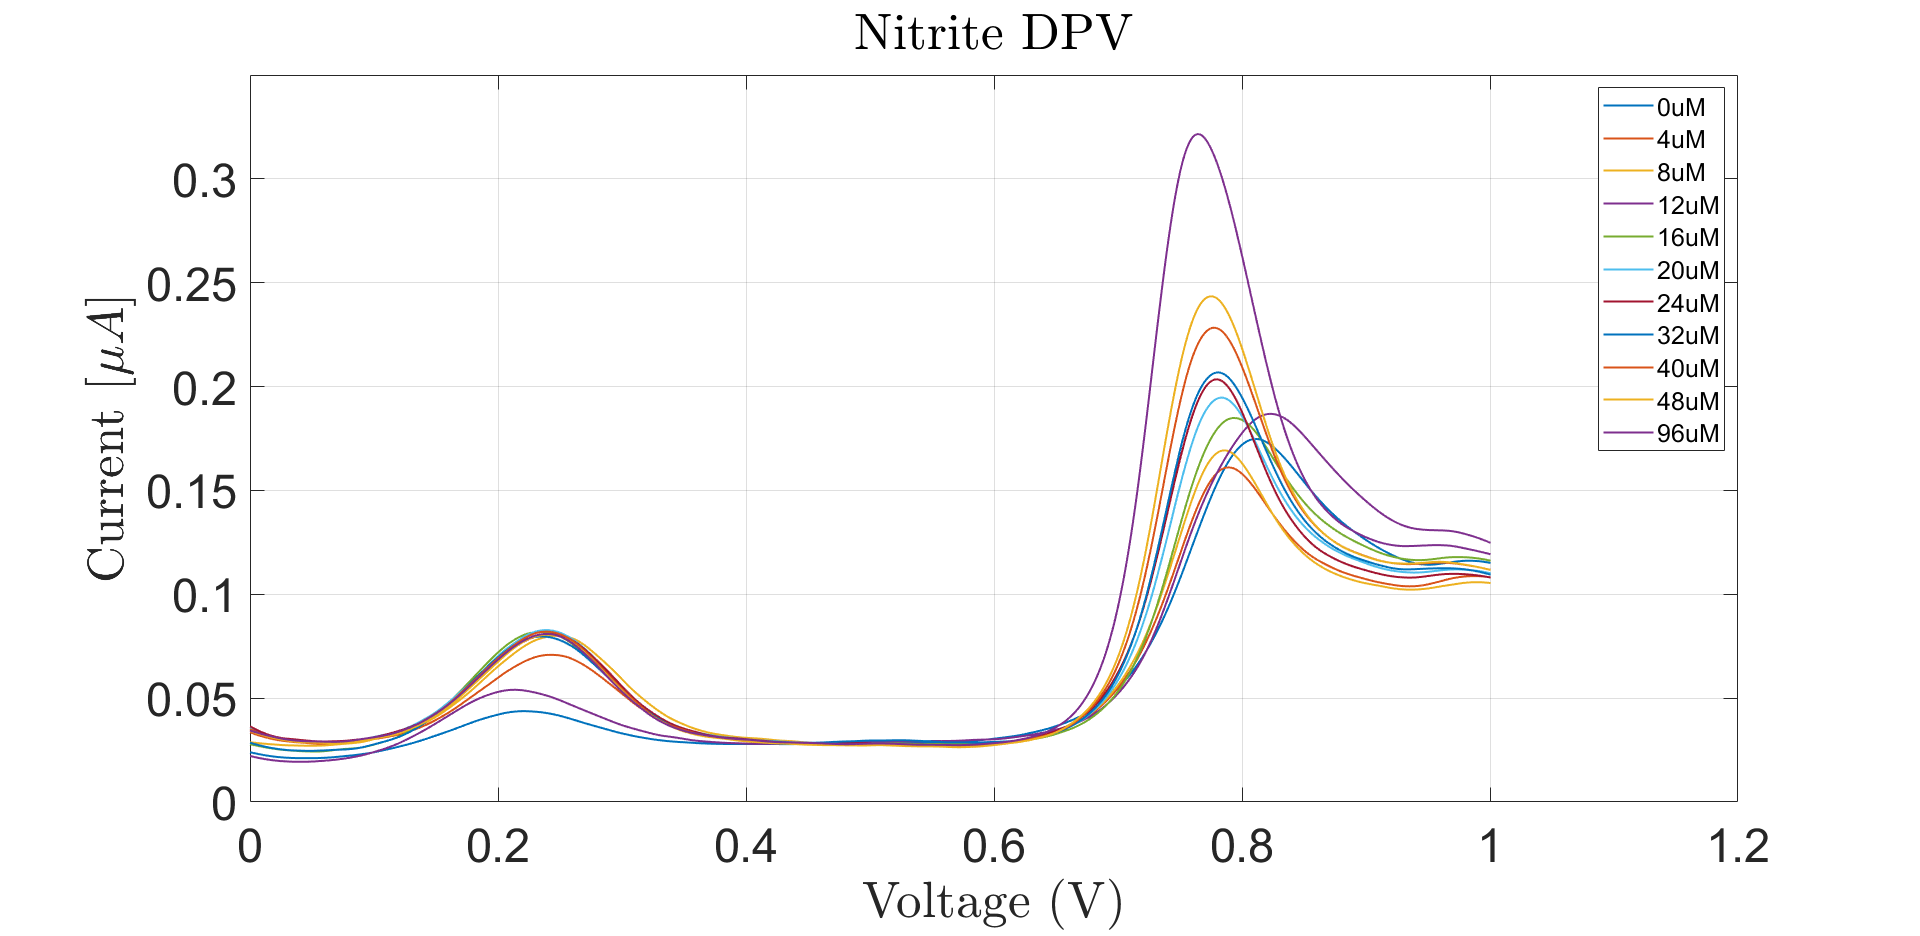
\includegraphics[width = 0.5\textwidth]{img/nitrite clean reus.png}
    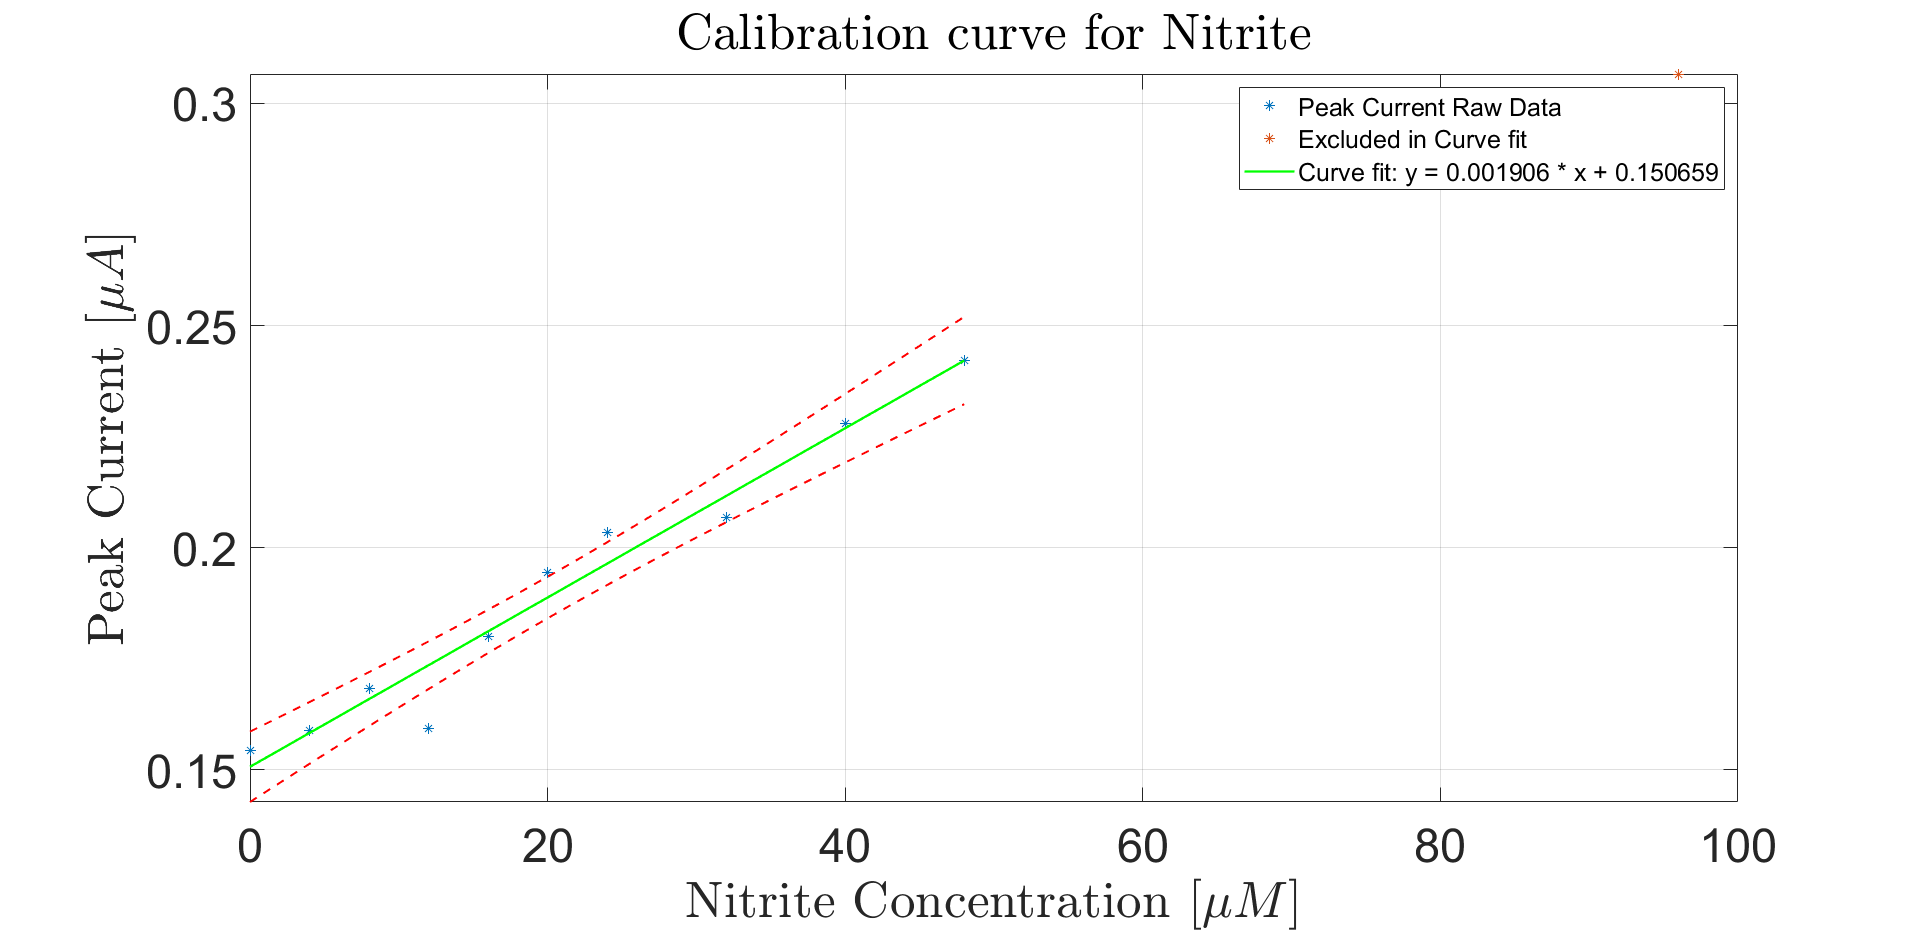
\includegraphics[width = 0.5\textwidth]{img/nitrite clean reus calibration.PNG}
     \caption{Voltammetry and calibration curve of nitrite in PBS - Reusable gold electrode. Calibration curve with regression line and 95\% CI} 
    \label{fig:nitrite_result_1}
\end{figure}

\subsubsection{Reusable gold electrode in PBS Solution and albumin}
\begin{figure}[H]
    \centering
    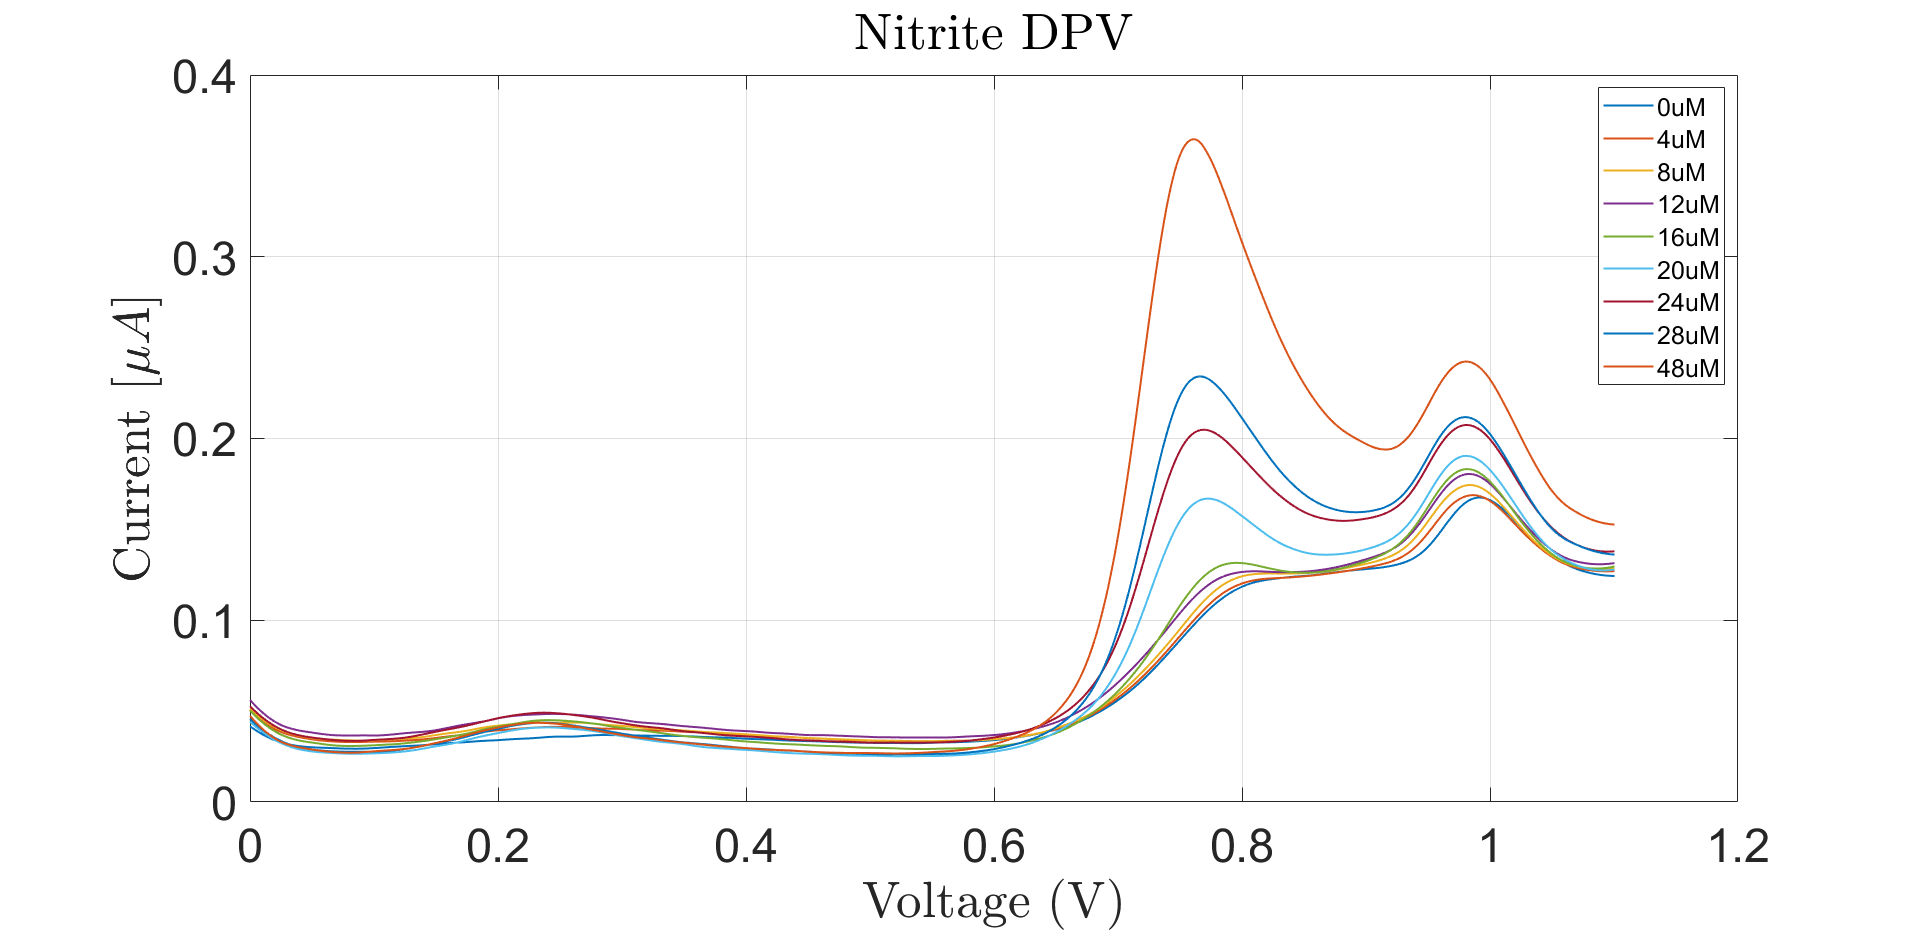
\includegraphics[width = 0.5\textwidth]{img/albumin reus.png}
    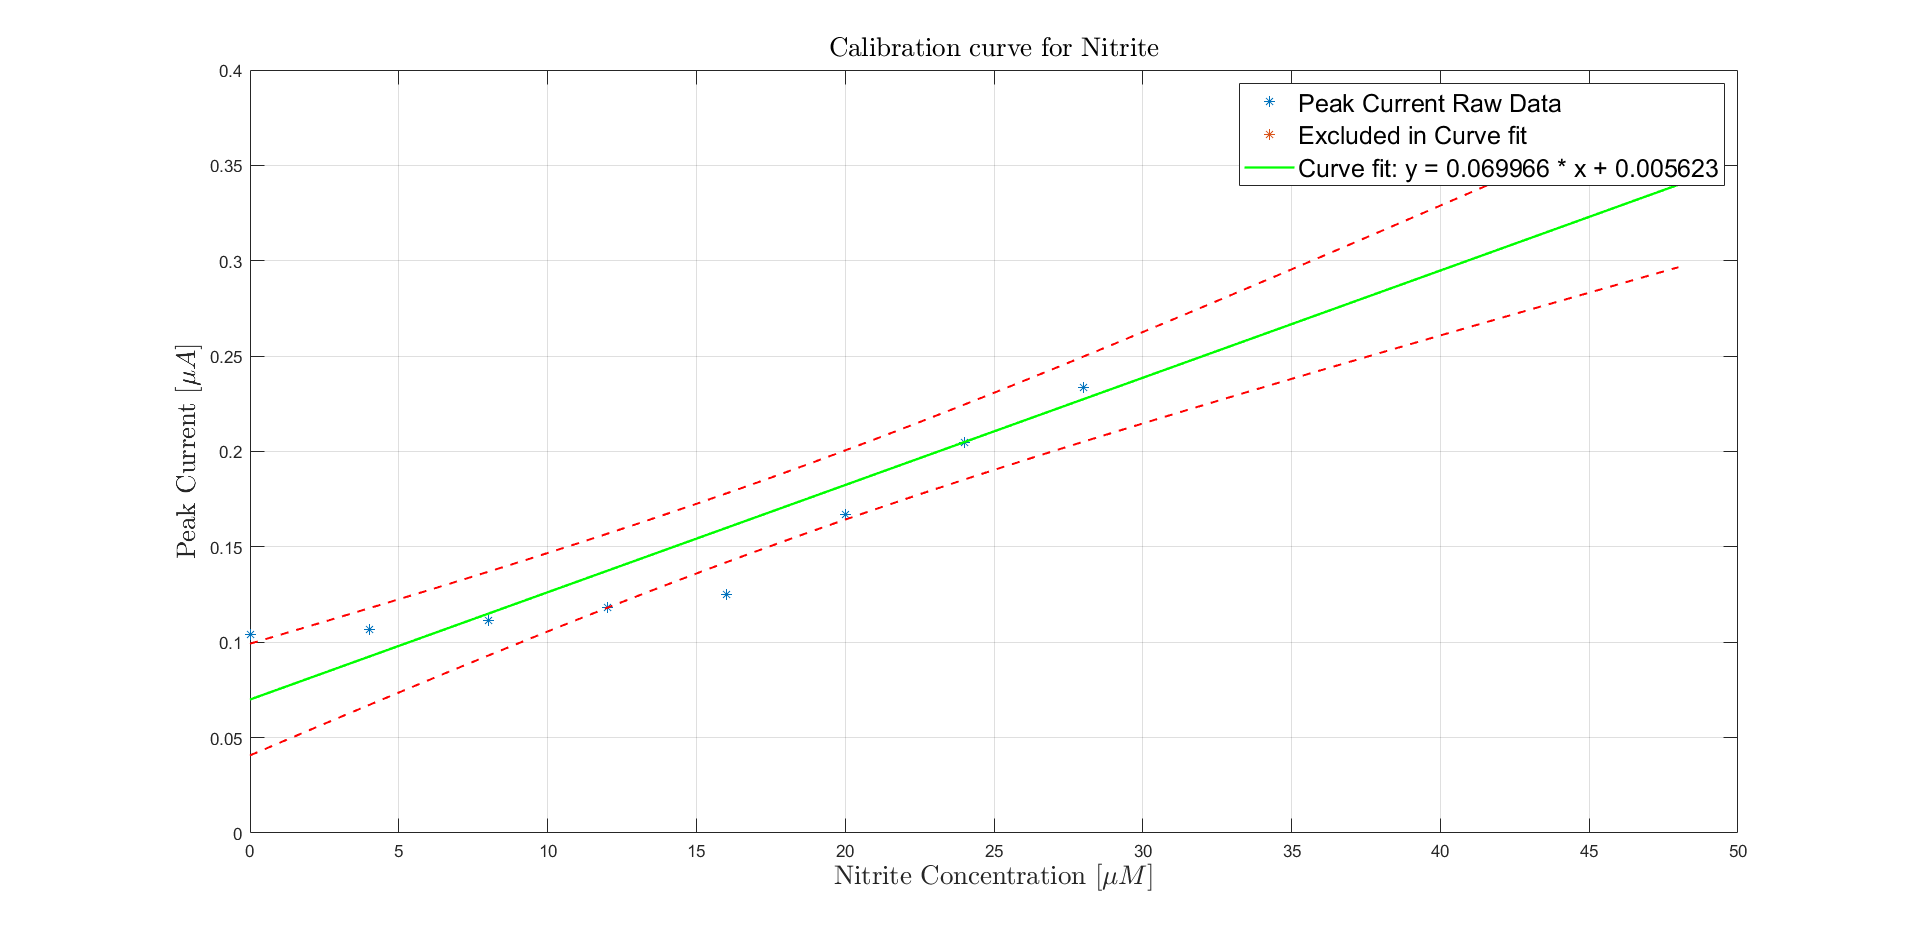
\includegraphics[width = 0.5\textwidth]{img/albumin reus calibration.png}
    \caption{Voltammetry and calibration curve of nitrite in PBS and 5.2 g/L albumin - Reusable gold electrode. Calibration curve with regression line and 95\% CI} 
    \label{fig:nitrite_result_2}
\end{figure}

\subsubsection{Disposable gold electrode in PBS Solution}
\begin{figure}[H]
    \centering
    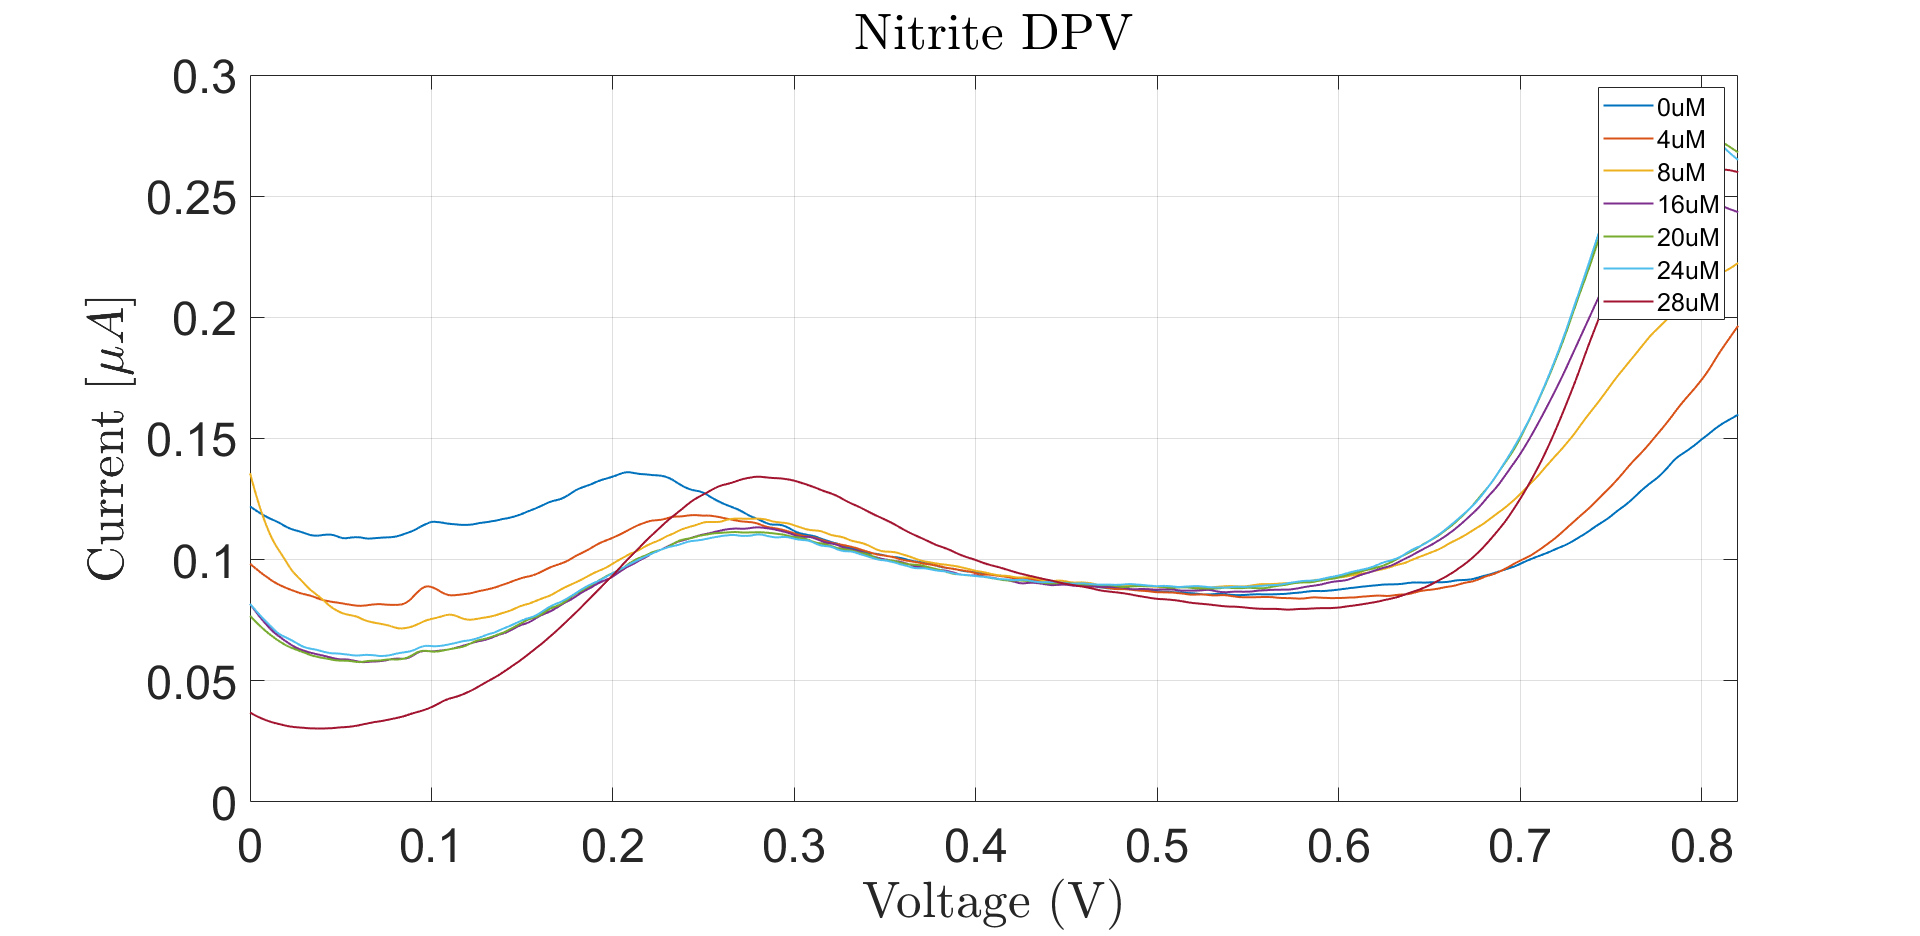
\includegraphics[width = 0.5\textwidth]{img/disp clean.png}
    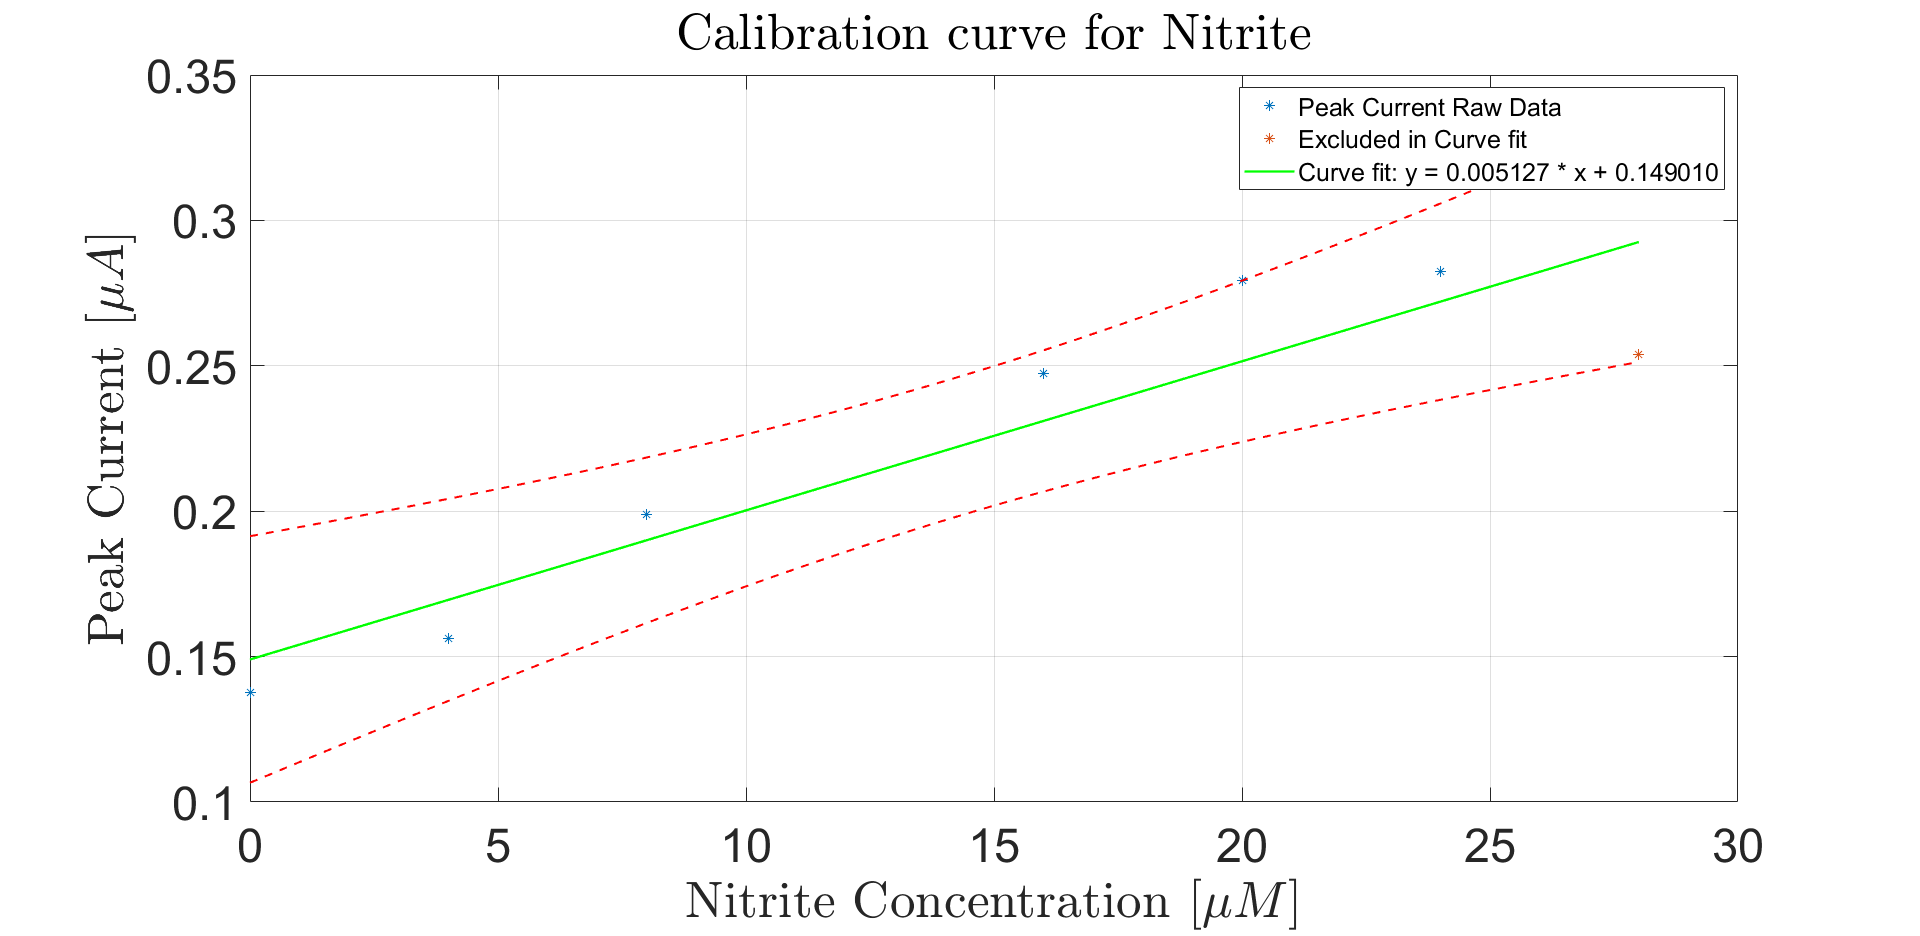
\includegraphics[width = 0.5\textwidth]{img/disp clean calibration.png}
    \caption{Voltammetry and calibration curve of nitrite in PBS - Disposable electrode. Calibration curve with regression line and 95\% CI}
    \label{fig:nitrite_result_3}
\end{figure}

\subsubsection{Disposable gold electrode in PBS Solution and albumin}
\begin{figure}[H]
    \centering
    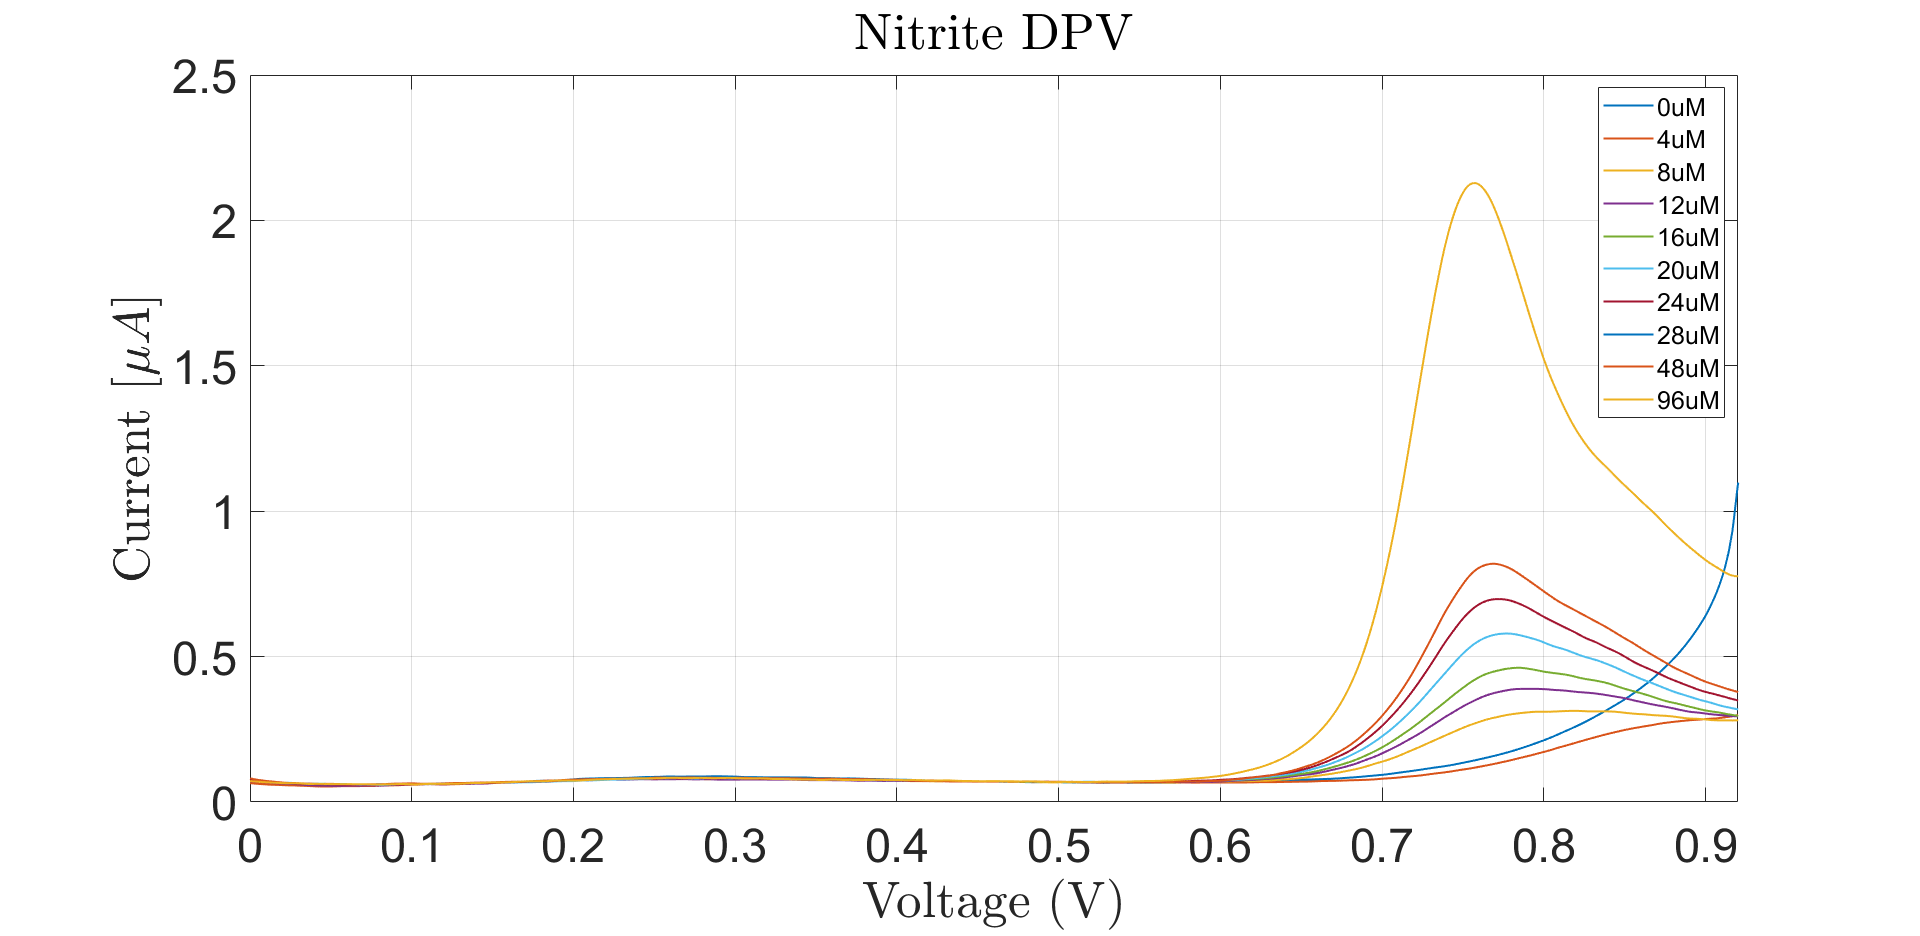
\includegraphics[width = 0.5\textwidth]{img/disp albumin.png} 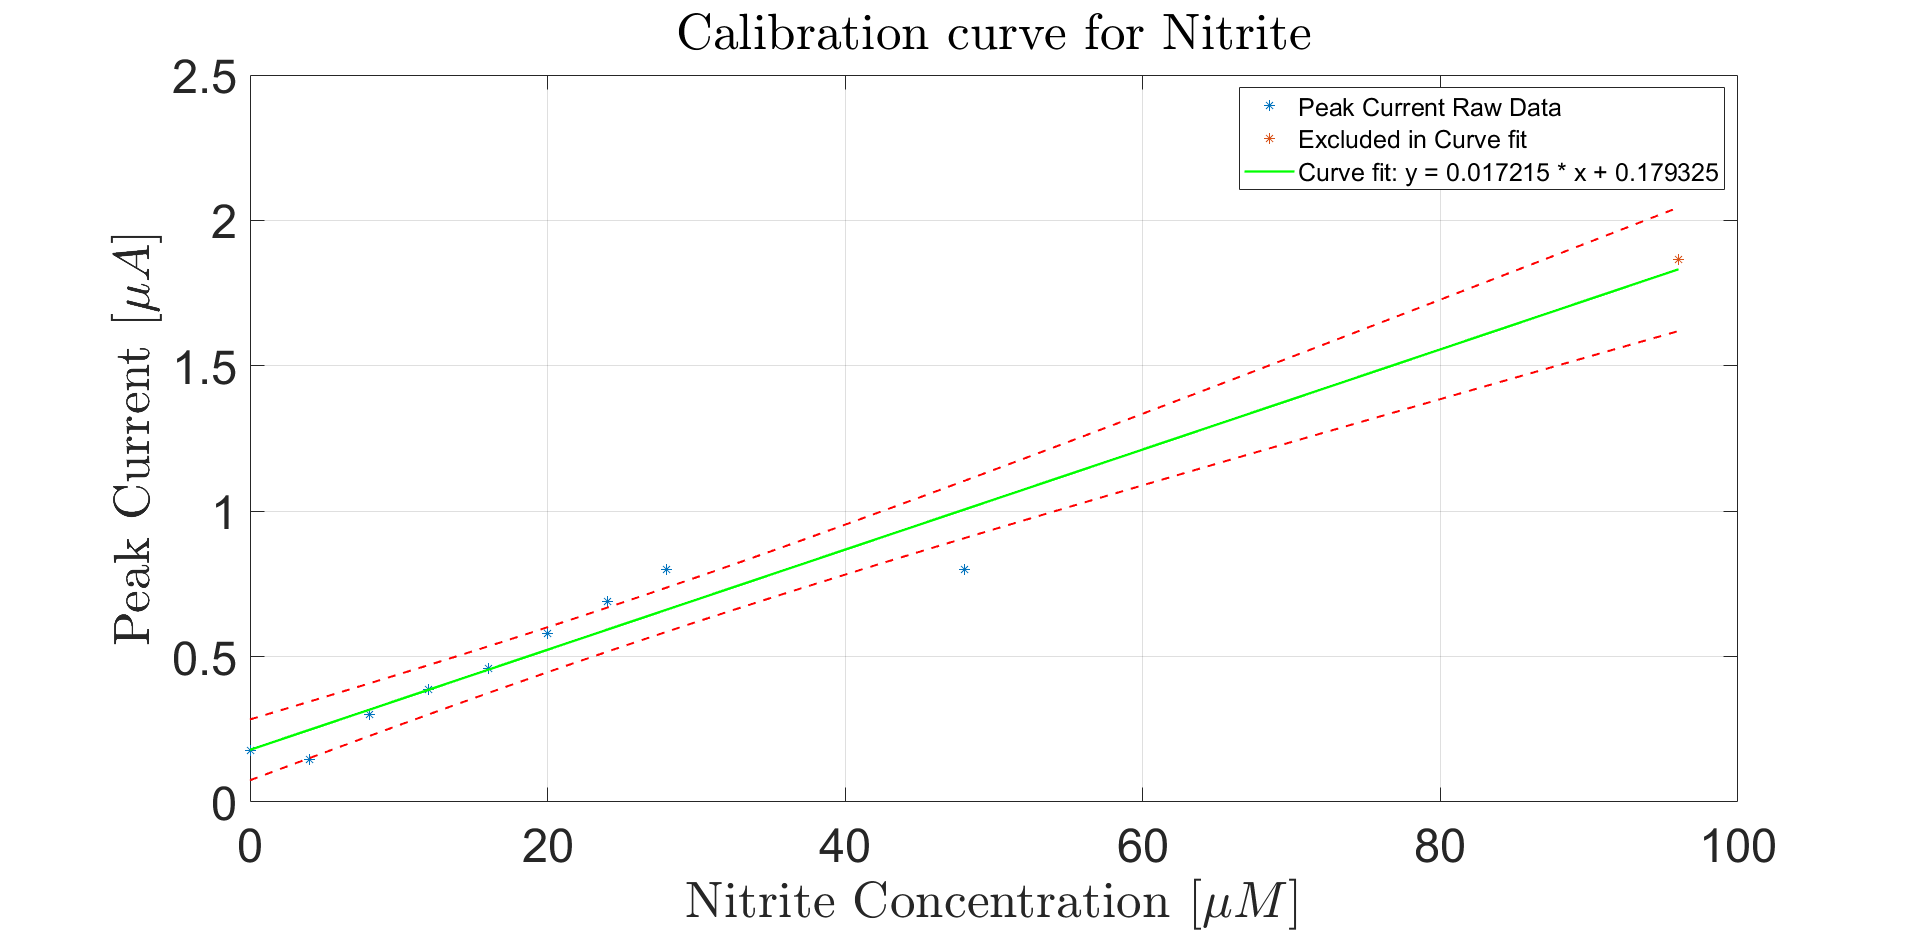
\includegraphics[width = 0.5\textwidth]{img/disp albumin calibration.png}
    \caption{Voltammetry and calibration curve of nitrite in PBS and 5.2 g/L albumin - Disposable electrode. Calibration curve with regression line and 95\% CI}
    \label{fig:nitrite_result_4}
\end{figure}

\subsubsection{Summary of calibration curves}
\begin{figure}[H]
    \centering
    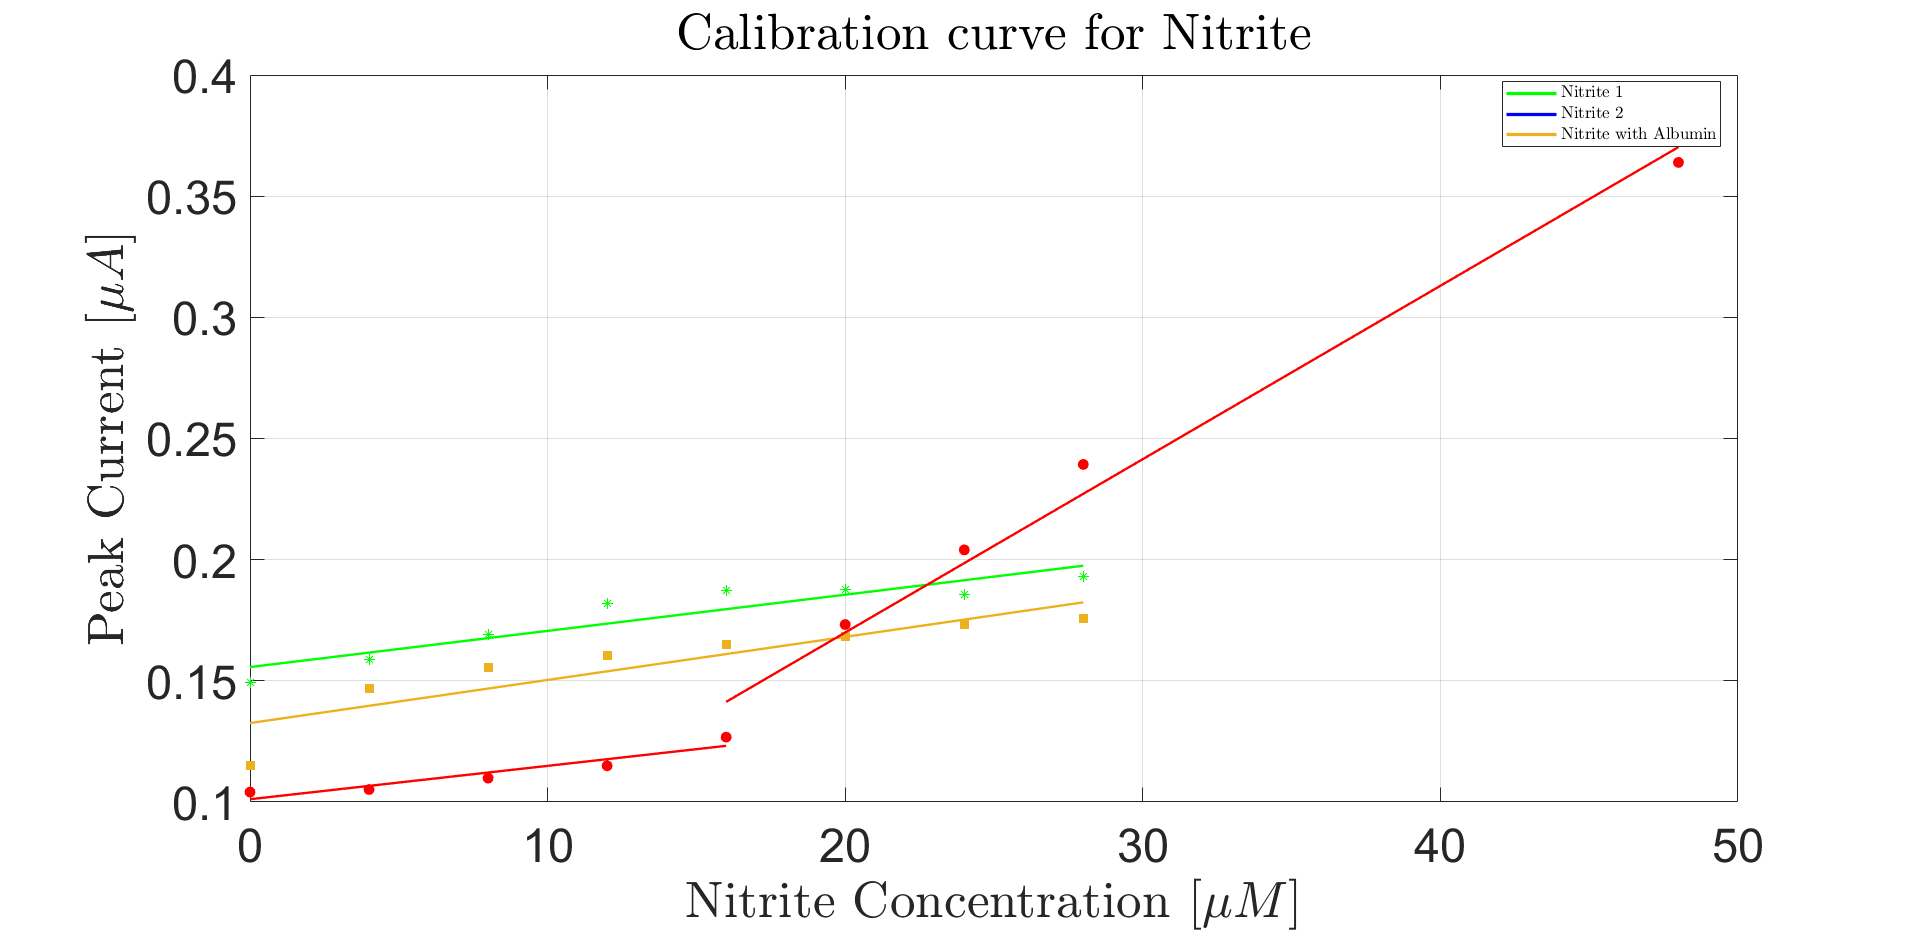
\includegraphics[width = 0.5\textwidth]{img/combinedreus new.png}
    \caption{Combined plot of reusable electrode calibration curve regression lines}
    \label{fig:nitrite_calibration_1}
\end{figure}

\begin{figure}[H]
    \centering
    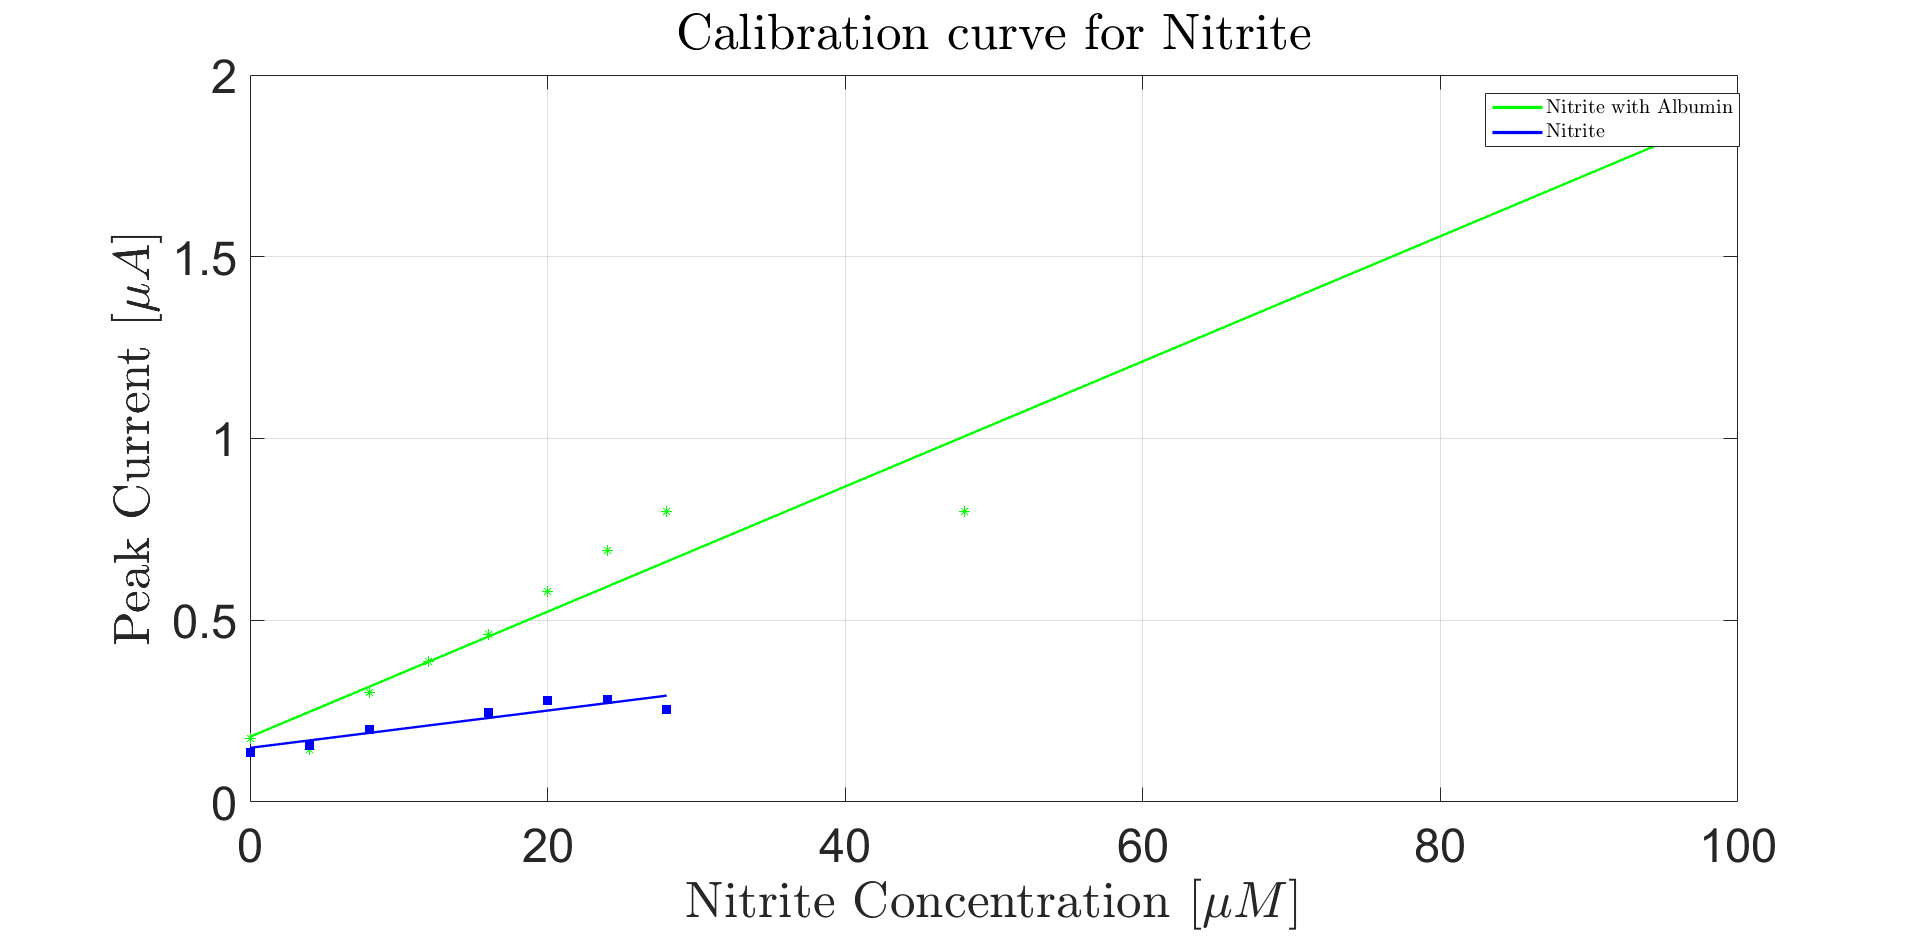
\includegraphics[width = 0.5\textwidth]{img/combined disp.png}
    \caption{Combined plot of disposable electrode calibration curve regression lines}
    \label{fig:nitrite_calibration_2}
\end{figure}

\begin{table}[H]
    \centering
    \begin{tabularx}{0.5\textwidth}{|p{1cm}|p{2.3cm}|c|c|c}\hline
    
    Nitrite & Sensitivity$\pm$SD /n\text{A} $\mu \text{M}^{-1} (s)$ & Intercept $(\mu \text{A})$ & LOD $(\mu \text{M})$ \\ \hline
    
    \textbf{1} & 1.5$\pm$0.5 & 0.156 &1.314  &   \\ \hline
    
    \textbf{2} & 1.9$\pm$.3 & 0.151$\pm$0.008 &  0.543&   \\ \hline
    
    \textbf{3} &1.8$\pm$0.8  &  0.133$\pm$0.5& 1.660 &   \\ \hline
    \end{tabularx}
    \caption {Sensitivity and LOD values for nitrite experiments}
    \end{table}
Current from increasing steps in E were measured and recorded. These were used to plot voltammograms with current as a function of voltage. Current drift was corrected and smoothed. Current of the highest peaks, between 0.7 and 0.8V in all graphs were recorded. Results obtained from each experiment are shown above.  A linear regression line with 95\% confidence intervals was constructed as shown in \autoref{fig:nitrite_result_1}, \ref{fig:nitrite_result_2}, \ref{fig:nitrite_result_3} and \ref{fig:nitrite_result_4}. Regression lines were then plotted alongside each other to compare gradients and SD between experiments, shown in \autoref{fig:nitrite_calibration_1} and \ref{fig:nitrite_calibration_2}.\\\\
DPV for measuring nitrite concentration using reusable gold electrodes in PBS was performed three times, returning similar traces each time (\autoref{fig:nitrite_result_1}). Performing linear regression produced curves with similar gradient, with no significant difference due to overlapping standard deviations.\\\\
Code used for plotting and processing collected data is documented in \autoref{app:nitrite_code}.
%=========================================================================================
\subsection{Hydrogen Peroxide Investigations}
Upon completing four cyclic voltammetry scans, the following voltage-current plot was obtained by taking the data from the last stable scan. A peak voltage at 0.209V and a trough voltage at -0.204V were observed when the applied sweep current reached 0.024mA and -0.321mA respectively, corresponding to the oxidation and reduction processes of PB. This process is an essential validation of the presence of PB in the experiment setup.  
\begin{figure}[H]
    \centering
    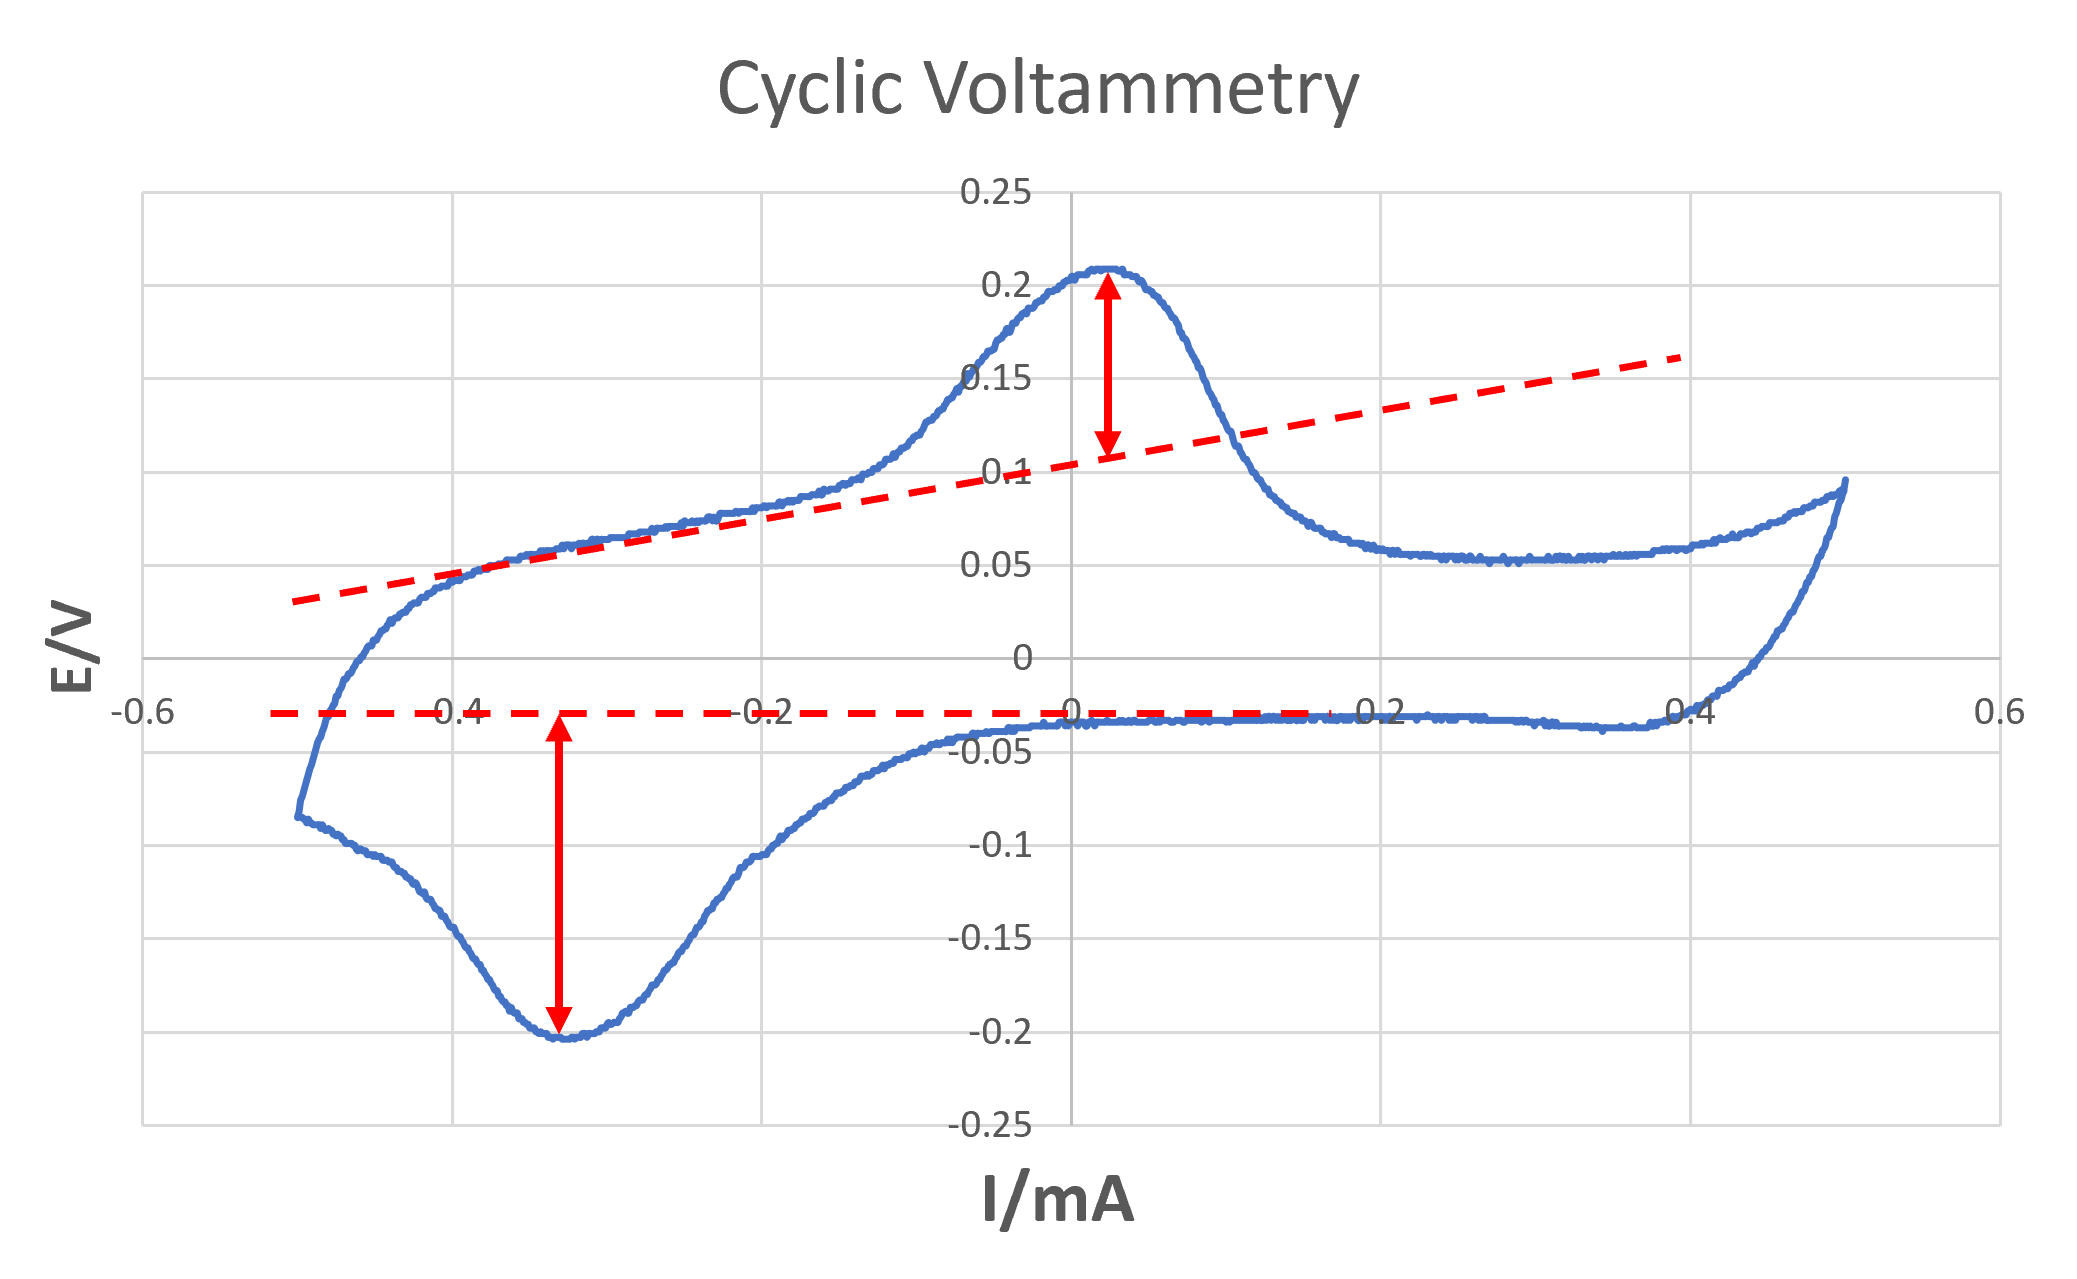
\includegraphics[width=.5\textwidth]{img/h2o2_cv.png}
    \caption{Cyclic voltammetry result}
    \label{fig:h2o2_cv}
\end{figure}
\noindent Chrono amperometry was performed following the cyclic voltammetry scan. The obtained results are shown in \autoref{fig:h2o2_amp}: hydrogen peroxide concentration ranged from 0 to M where stable current decreased with increased concentrations.
\begin{figure}[H]
    \centering
    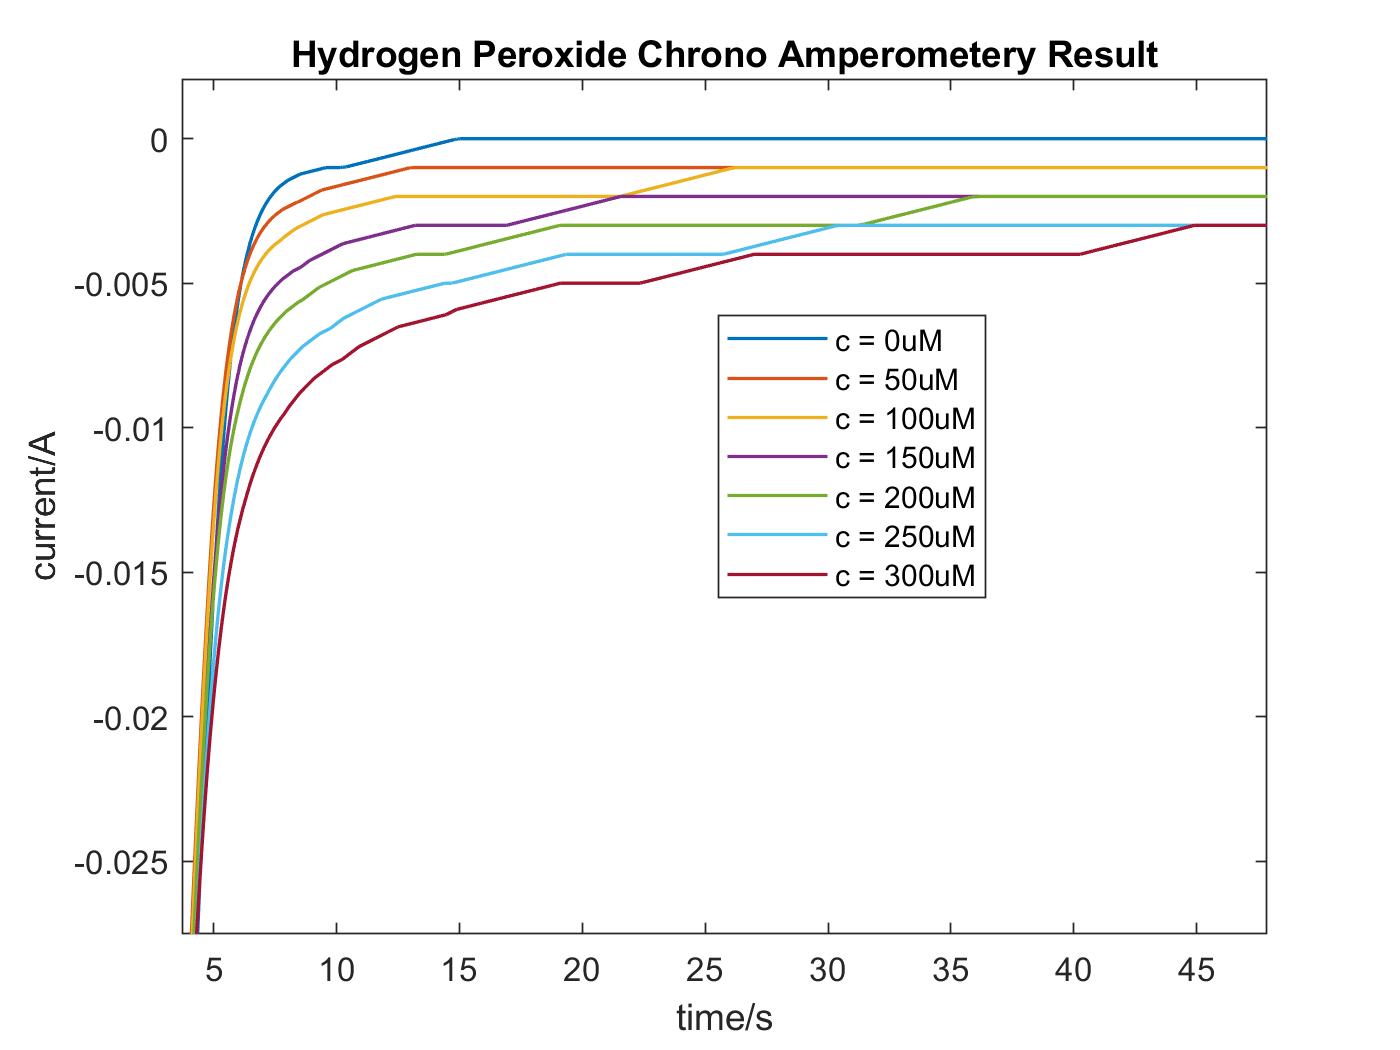
\includegraphics[width=.5\textwidth]{img/h2o2_amp.png}
    \caption{Cyclic voltammetry result}
    \label{fig:h2o2_amp}
\end{figure}
\noindent Coulometry serves as a powerful tool to amplify the current signal and reduce the noise through integrating the amperometry current data with respect to time \cite{Anson1966}. An improved Anson's equation with the consideration of edge-effect \cite{Flanagan1973} has been implemented to validate the experimental concentrations adopted in the electrode calibration curve, a detailed explanation and realisation of coulometry is shown in \autoref{app:h2o2_coulometry}. The result of coulometry is shown in \autoref{fig:h2o2_col} - the coulometry charge under each experimental concentration was plotted against the edge-corrected time, $(\sqrt{t}+\frac{1.92\sqrt{D}}{r}t)$ where $t$ is the sampling time over 180s. For each curve, a non-linear region was observed in the beginning, corresponding to the non-faradic charge due to double-layer charging and Prussian bule reduction. Following that, a major linear region appears almost immediately, indicating the charge transfer as the result of hydrogen peroxide reduction.
\begin{figure}[H]
    \centering
    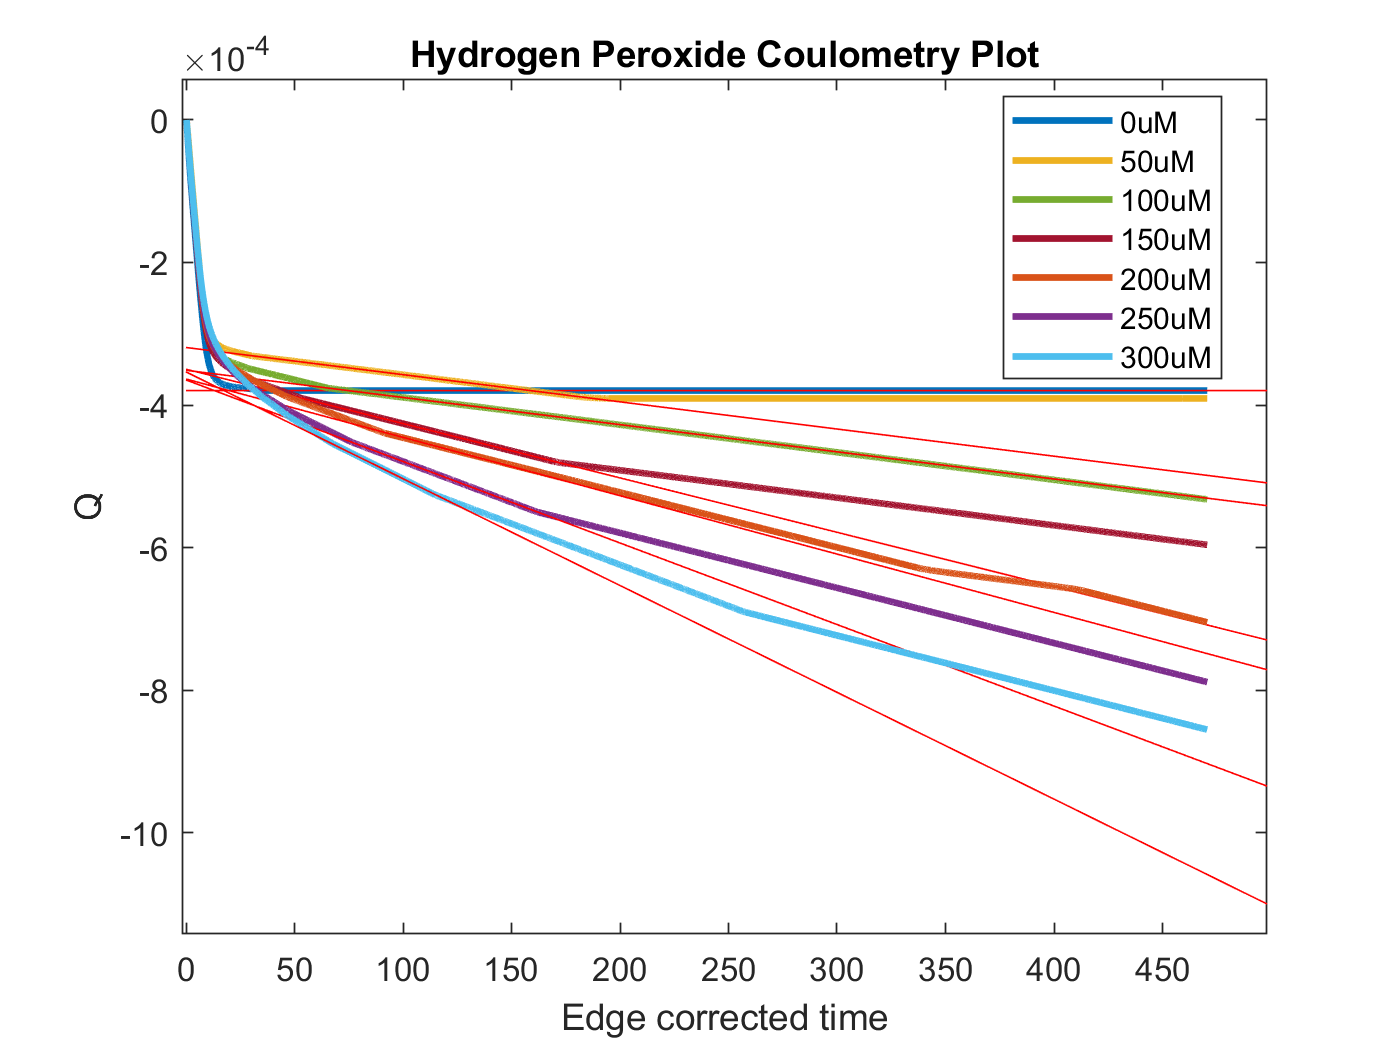
\includegraphics[width=.5\textwidth]{img/h2o2_coulometry.png}
    \caption{coulometry result}
    \label{fig:h2o2_col}
\end{figure}\vspace{-.8cm}
\noindent To perform curve fitting, 500 current and time data points in the linear region were selected from the coulometry curves for each concentration. The gradients of each linear-fitted line were reported in \autoref{tab:h2o2_col_res}, hence we calculated the theoretical concentrations based on the relation in \autoref{eqn:improved_anson}. Comparisons between the theoretical and experimental concentrations were then performed.
\begin{table}[H]
    \centering
    \begin{tabularx}{.45\textwidth}{|p{.12\textwidth}|p{.13\textwidth}|p{.126\textwidth}|}\hline
        Experimental concentration (uM) & Gradient of linear fitting line & Theoretical concentration (uM)  \\ \hline
        0   & -1.216e-19 $\pm$ 0 & 2.39e-19\\ \hline
        50  & -3.814e-07 $\pm$ 0 & 84.30\\ \hline
        100 & -3.814e-07 $\pm$ 0 & 84.30\\ \hline
        150 & -7.628e-07 $\pm$ 1e-10 & 168.5\\ \hline
        200 &  -8.189e-07$\pm$ 5e-9 & 181.0\\ \hline
        250 & -1.144e-06 $\pm$ 0 & 252.8\\ \hline
        300 & -1.499e-06 $\pm$ 3e-9 & 331.2\\ \hline
    \end{tabularx}
    \caption{Hydrogen peroxide coulometry results}
    \label{tab:h2o2_col_res}
\end{table}

%=========================================================================================
\subsection{Lactate Investigations}
\begin{figure}[H]
    \centering
    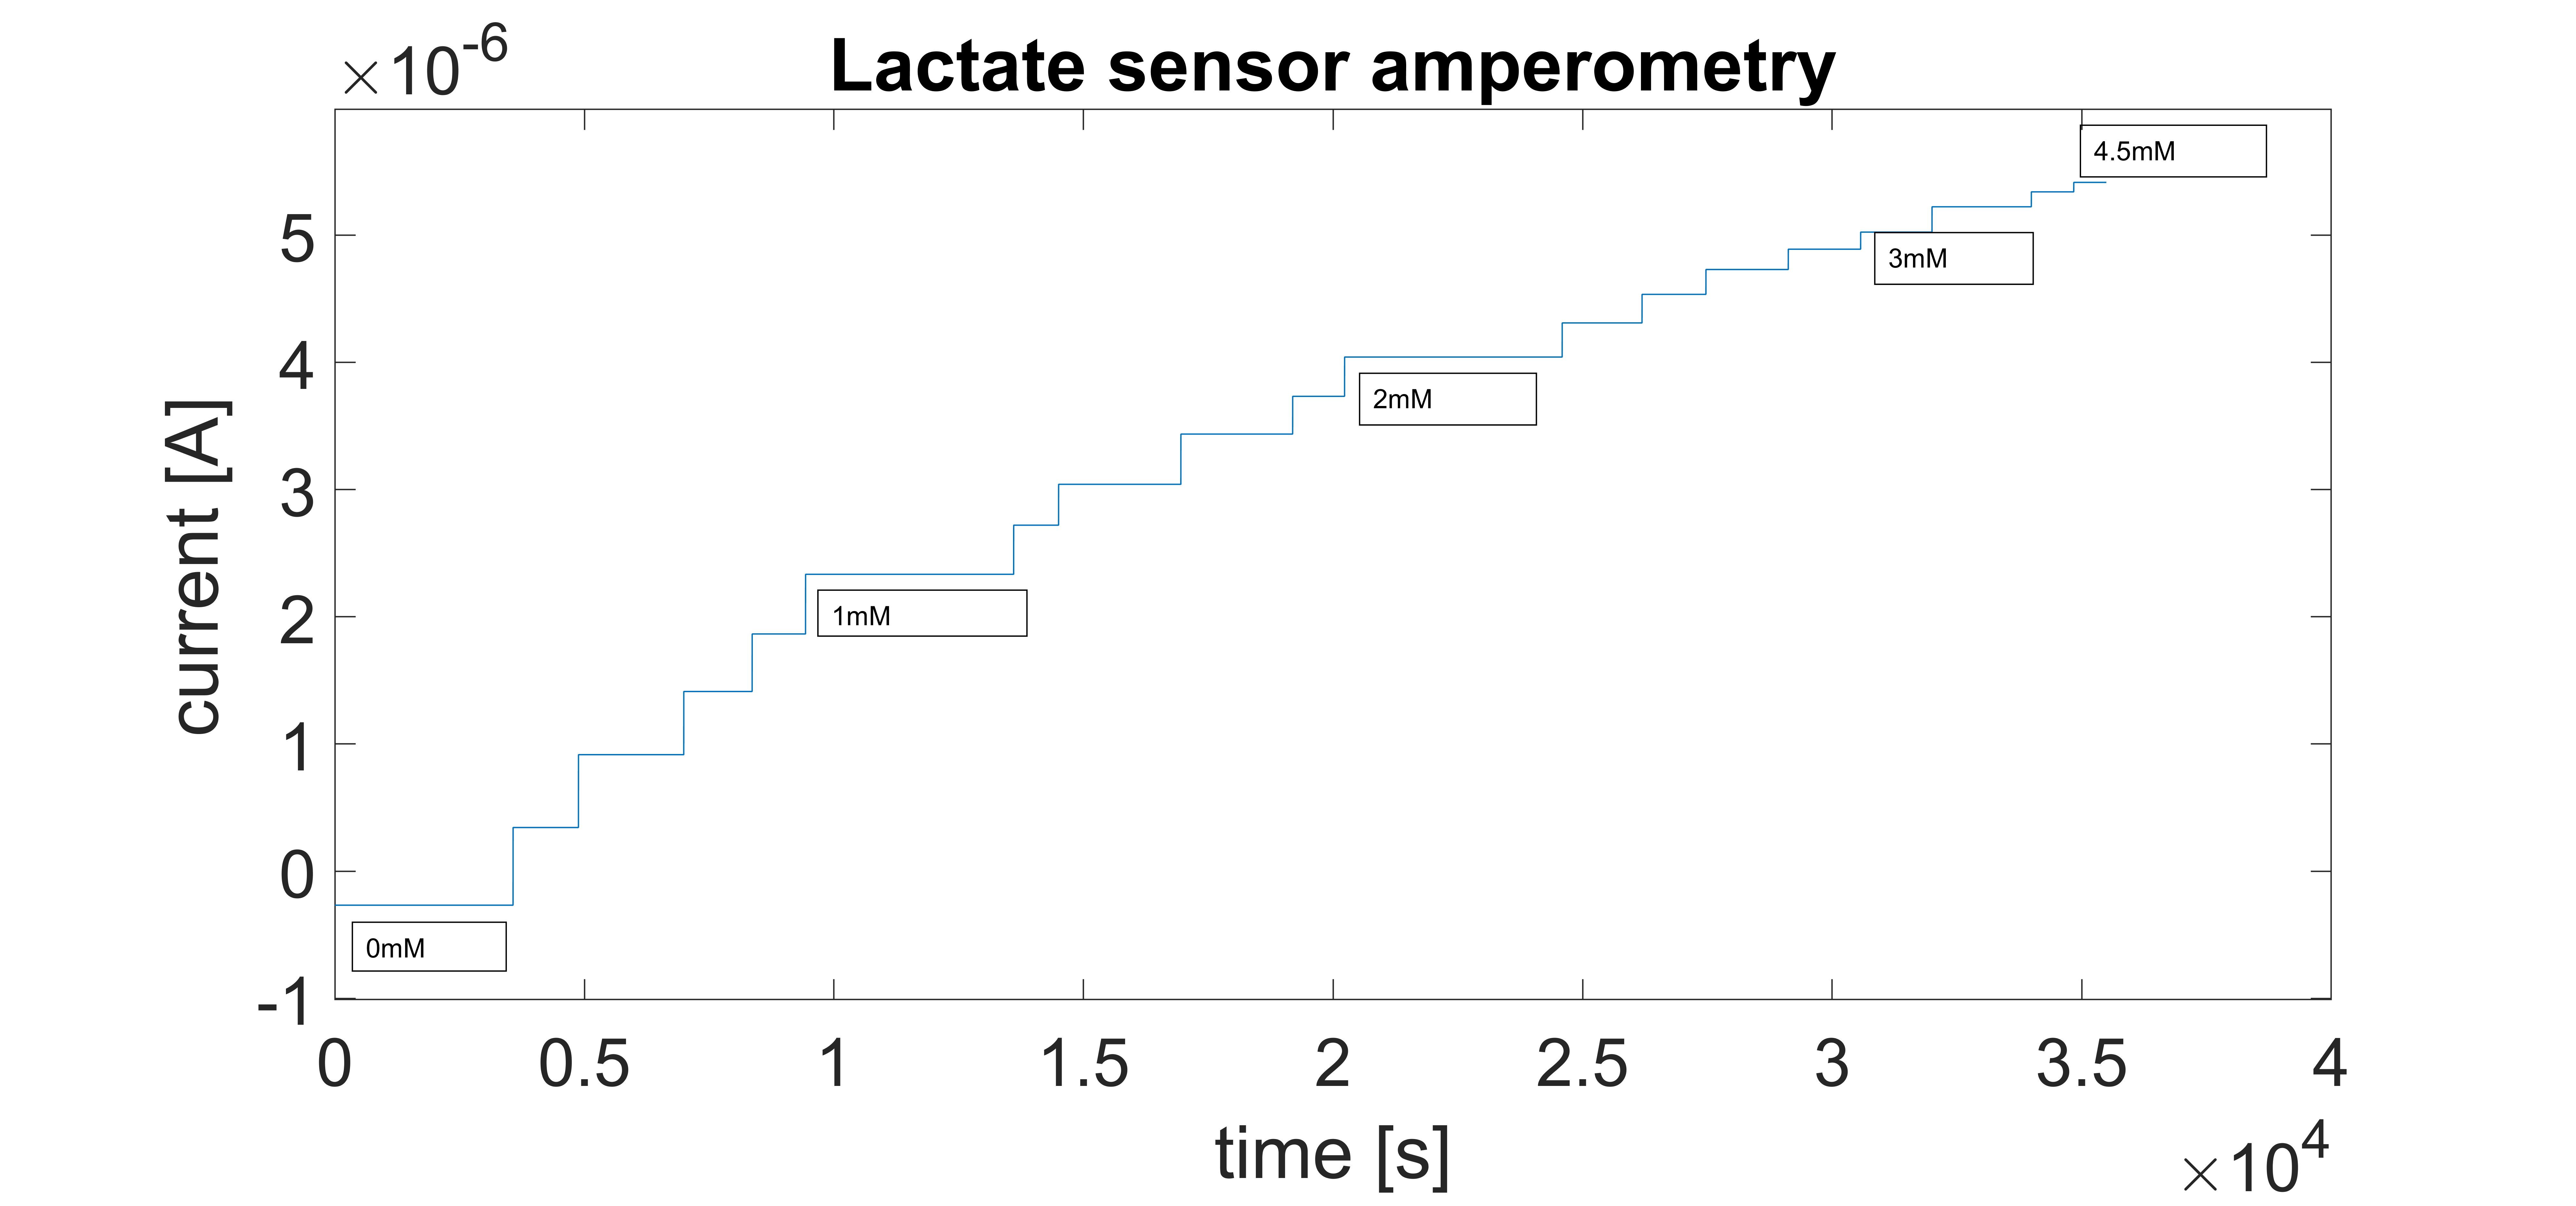
\includegraphics[width=0.5\textwidth]{img/Lactate_fig_1.png}
    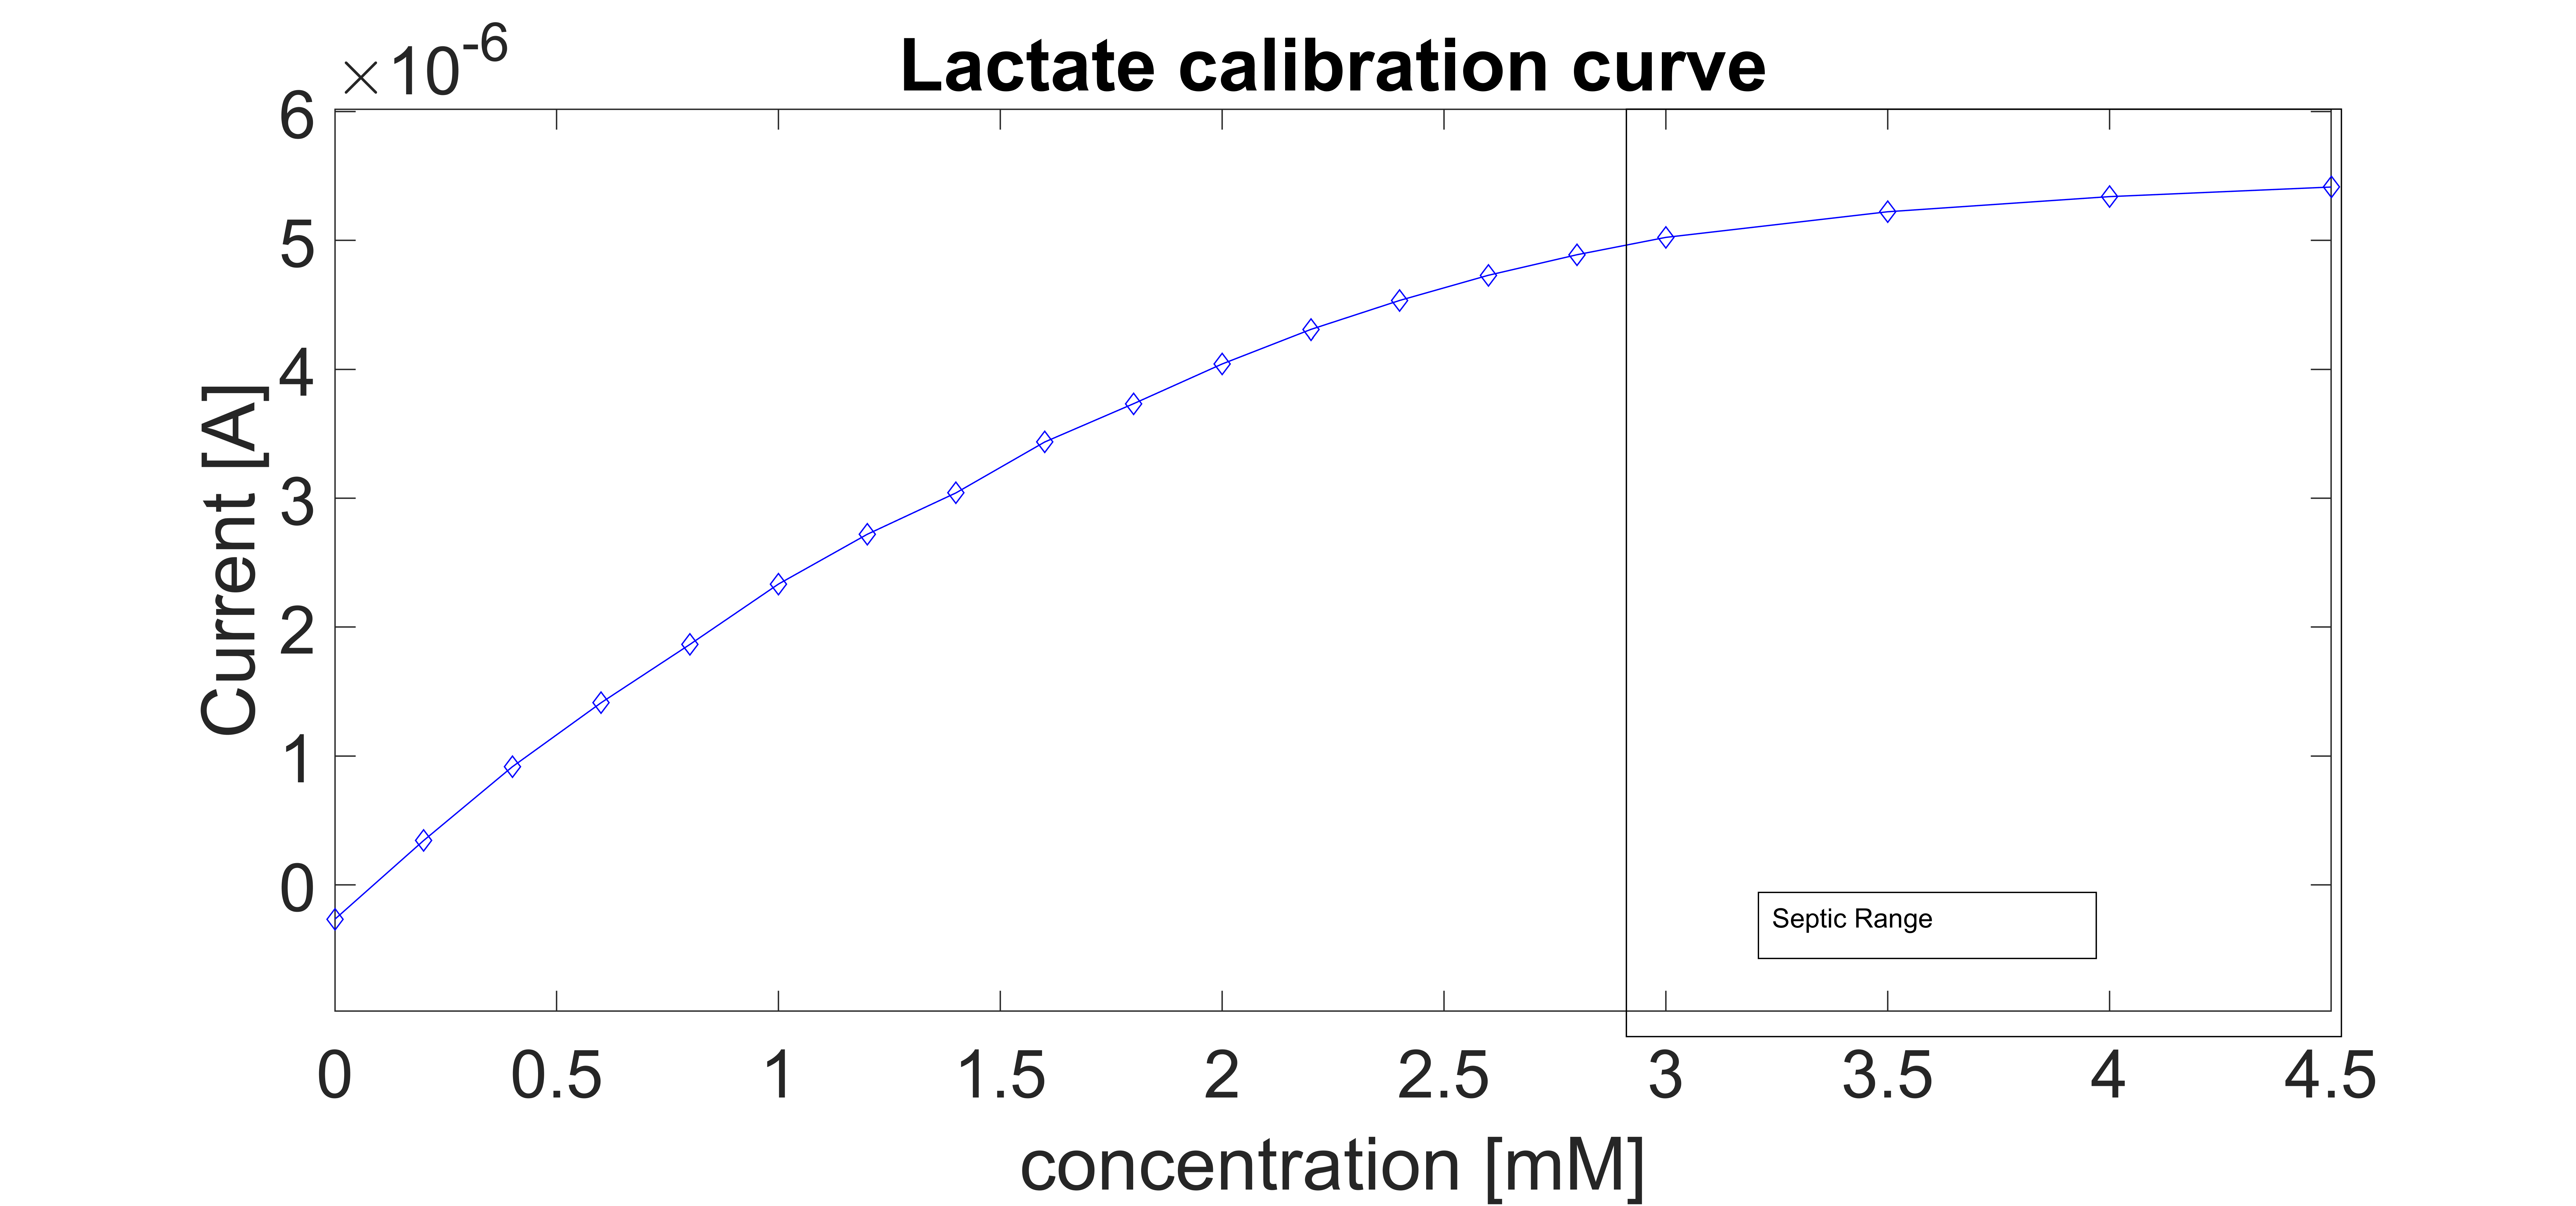
\includegraphics[width=0.5\textwidth]{img/Lactate_fig_2.png}
    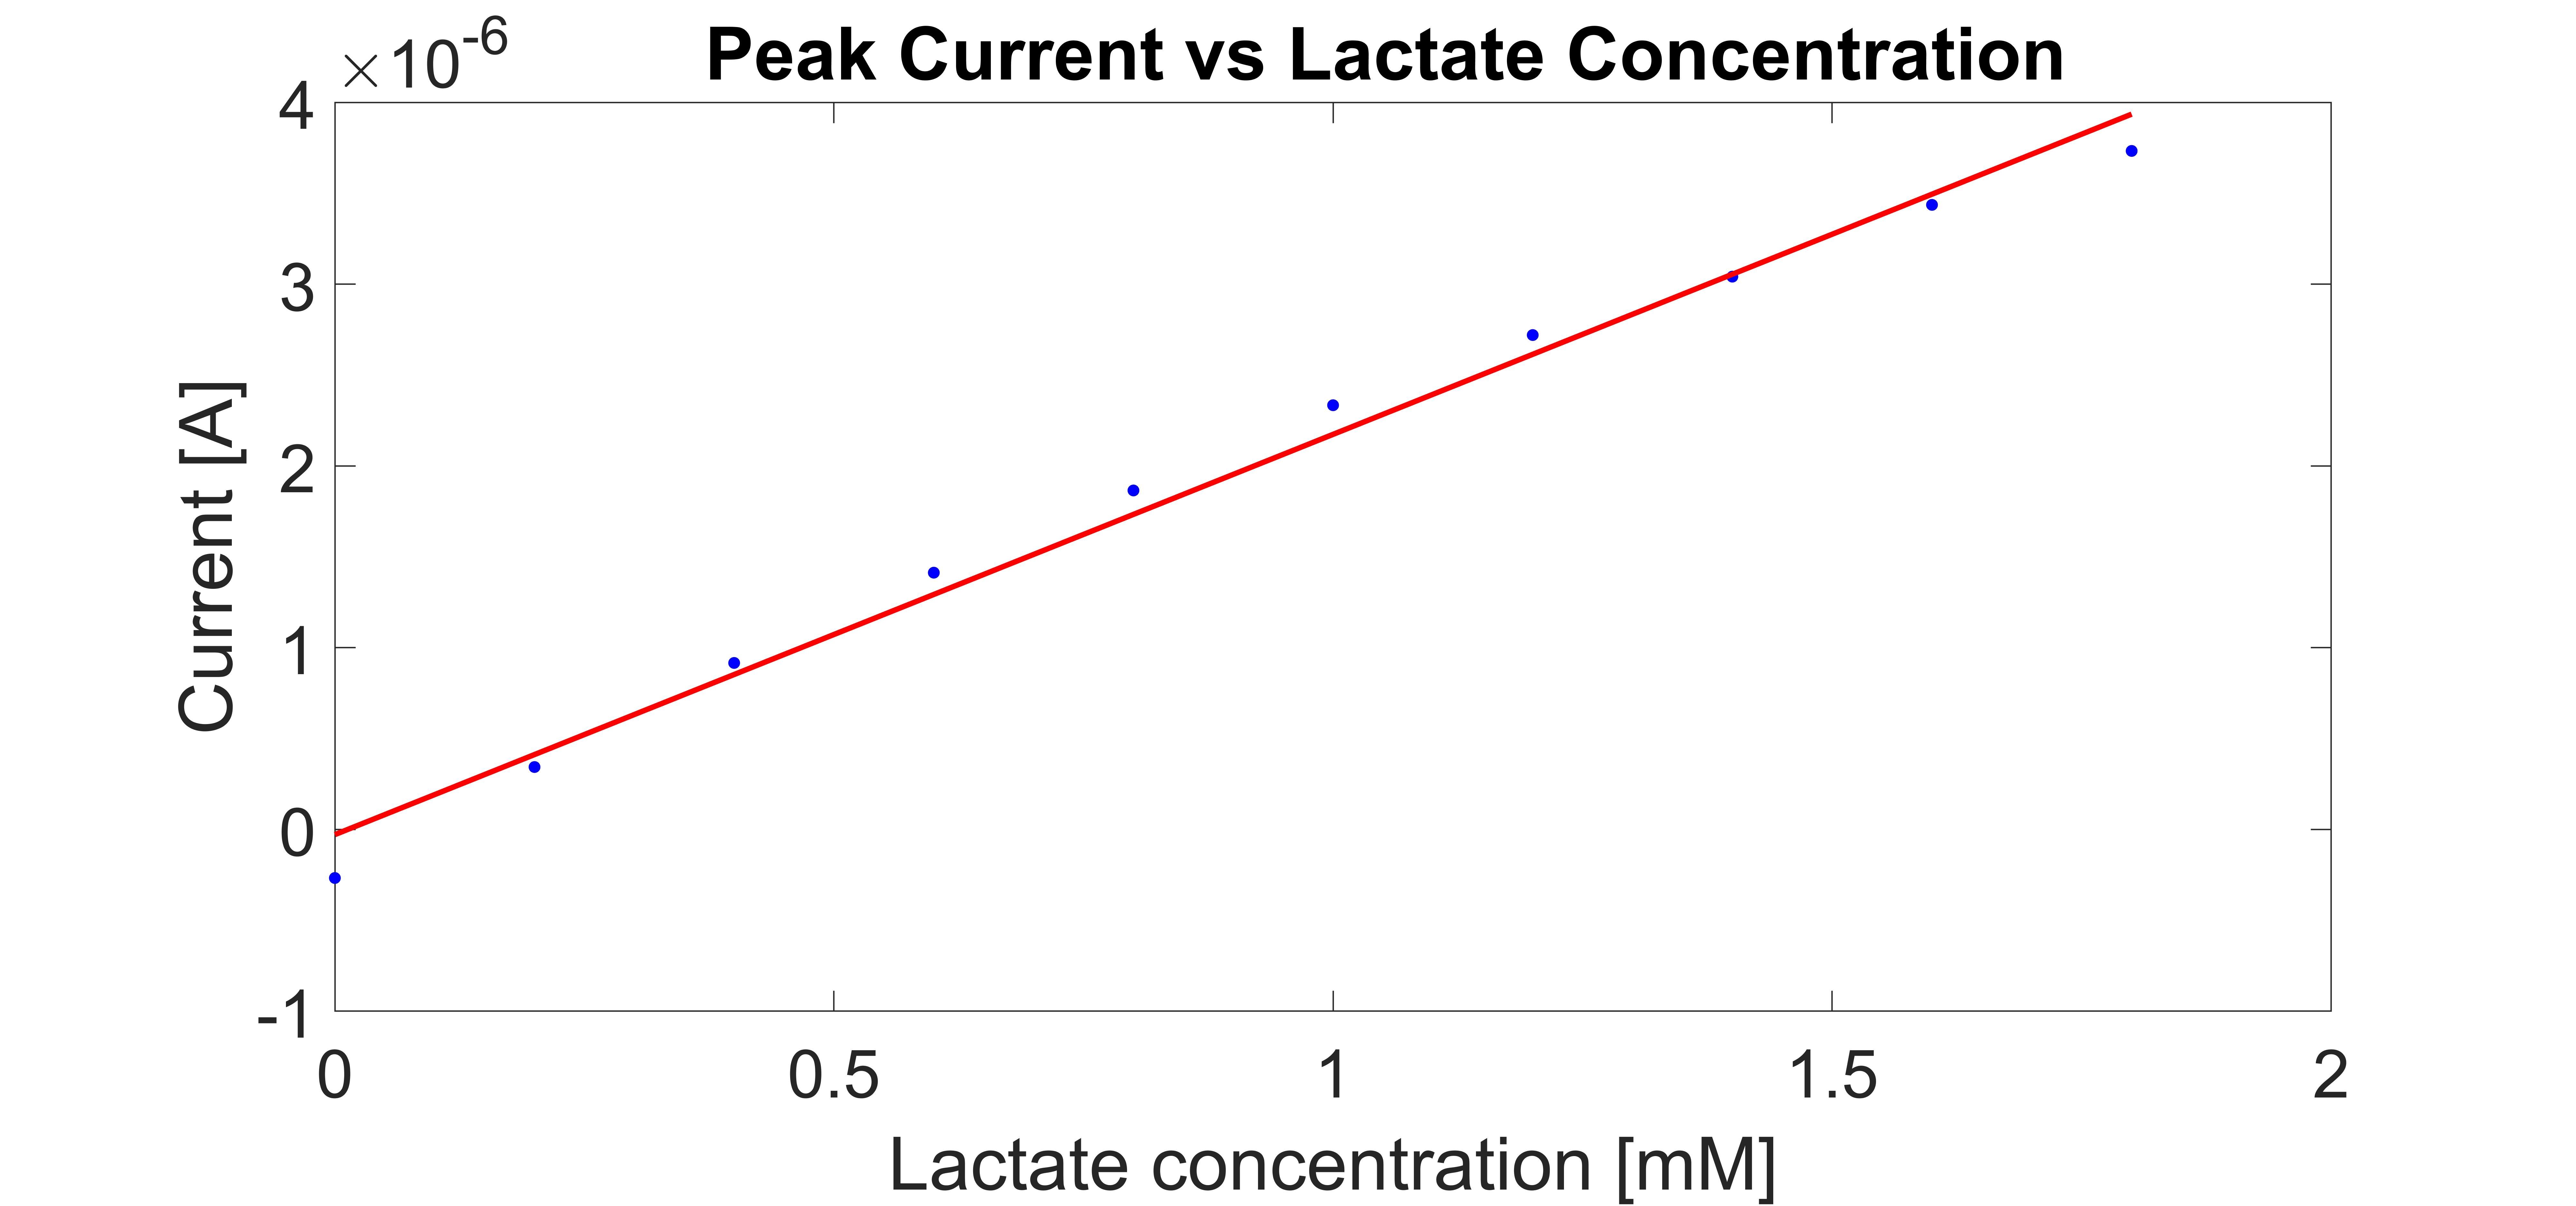
\includegraphics[width=0.5\textwidth]{img/Lactate_fig_3.png}
    \caption{(From top to bottom)(a)Amperometry plot of lactate additions from 0-4.5mM/L lactate solution. (b) Calibration curve of current vs concentration. (c) Linear approximation for the calibration data up to 2mM/L}
    \label{fig:lactate_result}
\end{figure}
In \autoref{fig:lactate_result}(a), the change in current can be observed after each addition of lactate. An average current for each step interval was taken and plotted against time. The time intervals indicate how long the readings took to stabilise, this is of no importance in our conclusions, rather this was due to movement of apparatus or noise. In \autoref{fig:lactate_result}(b) the average currents were then plotted against the lactate concentration  to produce calibration curves as seen in \autoref{fig:lactate_result}(b). Up to a concentration of 2mM/L, the current rises linearly with concentrations shown in \autoref{fig:lactate_result}(c). By plotting the line of best fit, it can be estimated that current increases by 5.48mA for every 1mM additions. \\\\ 
Beyond 2mM/L we still see an increase in current but it is no longer linear and the increase is more shallow at an average increase of  1.20mA per mM of lactate added, a definite plateau indicating poor detection capability in this range. 
\subsection{Multiexponential Rate Extraction on Simulated data}
\vspace{-1cm}
Due to the absence of aptamer data, we test our numerical inverse Laplace multiexponential decomposition using simulated data with superimposed noise. In Plaxco's chronoamperometric study for the detection of Tobramycin, rate constants 100$s^{-1}$ and 500$s^{-1}$ were obtained with no target and saturating target concentration \cite{arroyo2018subsecond}. We have simulated a noise of 10dB, such that it emulates the noise in our instrumentation. In all our simulations, we test with equal values of coefficients [A] and [AT].\\\\
There are three tunable parameters in the algorithm to optimise the solution for the inverse laplace spectra $\mathbf{G}(k)$. 1) The solution space for $\mathbf{G}(k)$. 2) Resolution of points in the solution space. 3) The value of $\alpha$, the regularizer. \\\\
We constrain the solution space between $k = 10s^{-1}$ and $k = 800s^{-1}$). We ran a parameter analysis using alpha to determine an optimum value that provided the most accurate solution (\autoref{alpha}). At smaller values of $\alpha$ ($\alpha = 0.1$), the output waveform is spiky. At larger values of $\alpha$, the inverse laplace is excessively smoothed, where the peaks are widened. we therefore chose the $\alpha = 1$, due to the smooth output waverform, without widening the peaks of $\mathbf{G}(k)$. We therefore use $\alpha = 1$ in future simulations with the inverse laplace method, as it produces the most accurate and representative results, out of all the values of alpha tested.\\\\
Testing the algorithm on simulated double exponential data (with rates $k_{A}$ = 100$s^{-1}$ and $k_{AT}$ = 500$s^{-1}$) with the presence of noise, we can observe two distinct peaks centred at the two relevant rate constants of the signal (Figure \ref{multiexp}). In order for the algorithm to test the rate constants for the target bound and target unbound aptamer, we need to assess the ability of the algorithm to resolve rate constants that could potentially be closer. We find that the resolution is accurate for $k_{A}$ = 150$s^{-1}$ and $k_{AT}$ = 450$s^{-1}$ (\autoref{multiexp_2}), but as the two rate constants are brought closer together, the peaks overlap, forming a bimodal distribution (Fig. \ref{multiexp_3}). At ($k_{A}$ = 250$s^{-1}$ and $k_{AT}$ = 350$s^{-1}$ (\autoref{multiexp_4})), only a single peak is observed. The ability for this numerical inverse Laplace method to resolve rates that are close together is affected by the presence of noise in the raw signal, and the resolution of $\mathbf{G}(k)$ defined. More realistic experimental data would help characterise the nature of the noise and resolution of the $\mathbf{G}(k)$ is limited by computational time.\\\\
%\belowdisplayskip=0pt\relax
%\begin{equation}
%     f'(t) = awgn(f(t),SNR = 10dB)
%\end{equation}
To obtain the coefficients of the each exponential decay, we can use the normalised intensity values that is output from the numerical inverse Laplace (\autoref{multiexp}), or take the central value of the two peaks for the rate constant, and use the numerical inverse laplace algorithm to extract the coefficients.
\begin{figure}[H]
    \centering
    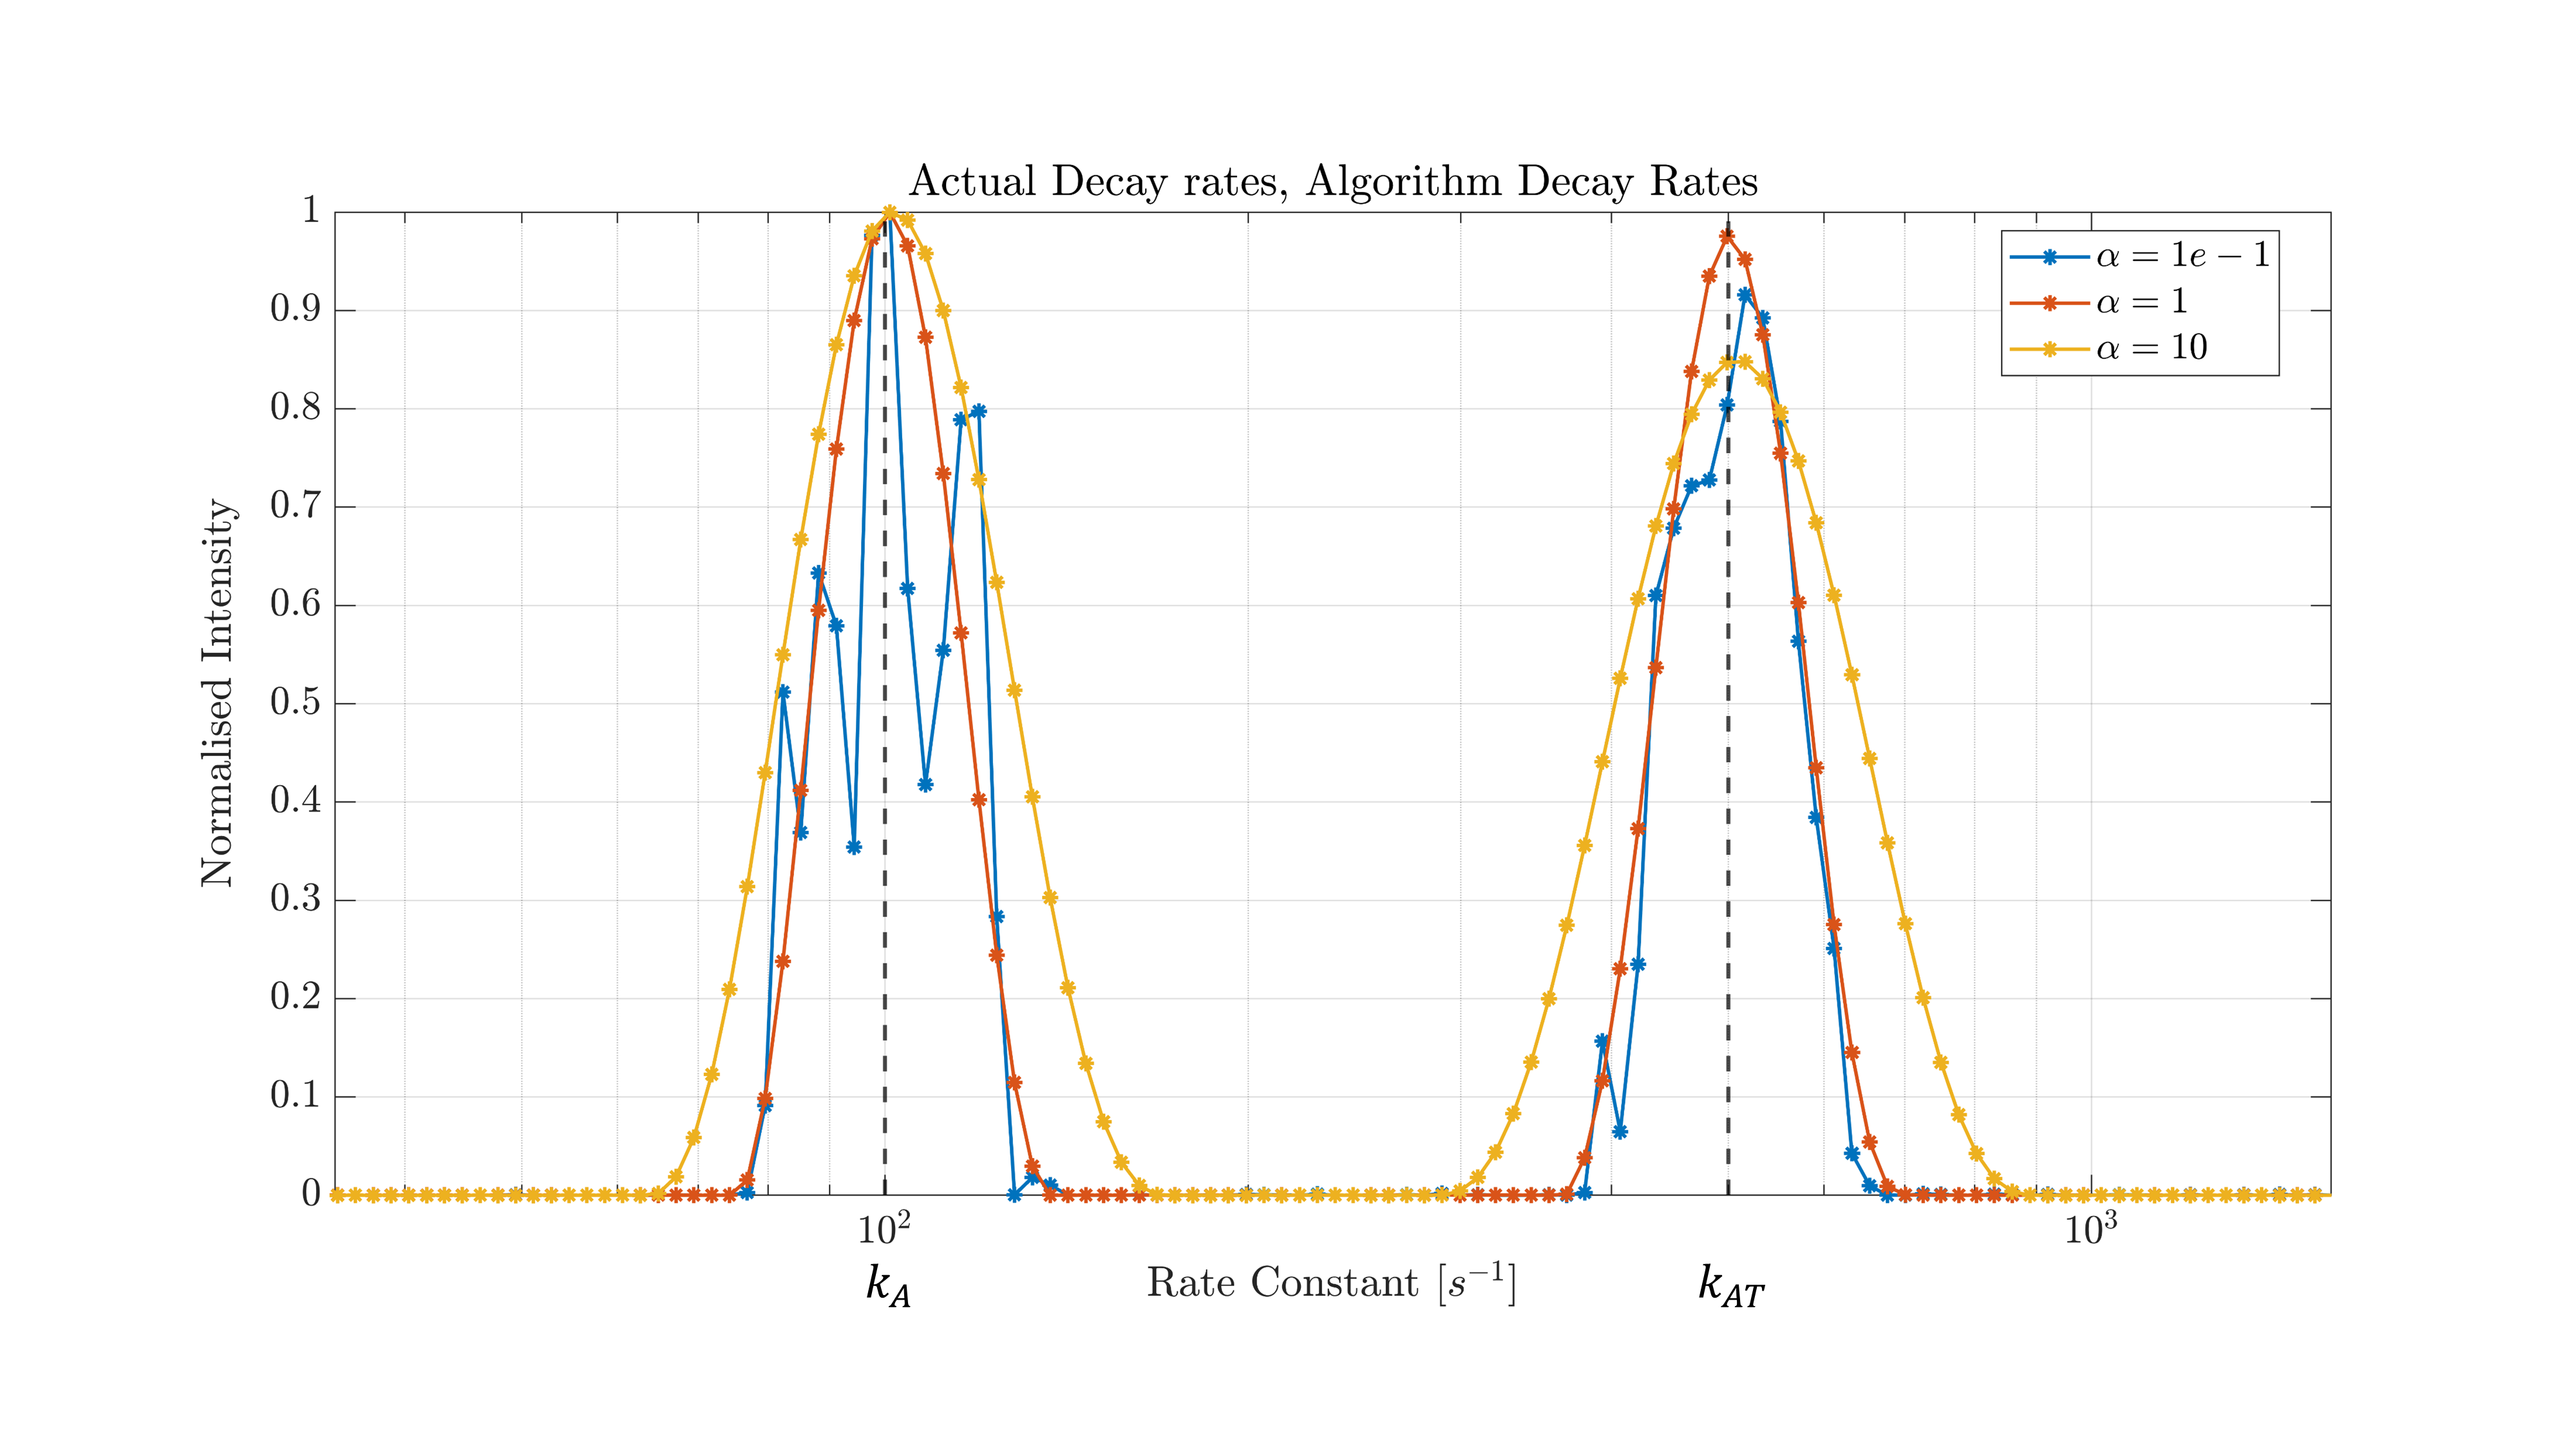
\includegraphics[width = 0.5\textwidth]{img/alpha_testing_annotate.png}
    \caption{Parameter sensitivity analysis using three values of $\alpha$. $\alpha = 1$ provided the best solution that represented the intrinsic rate constants present in the raw signal.}
    \label{alpha}
\end{figure}
\begin{figure}[H]
    \centering
    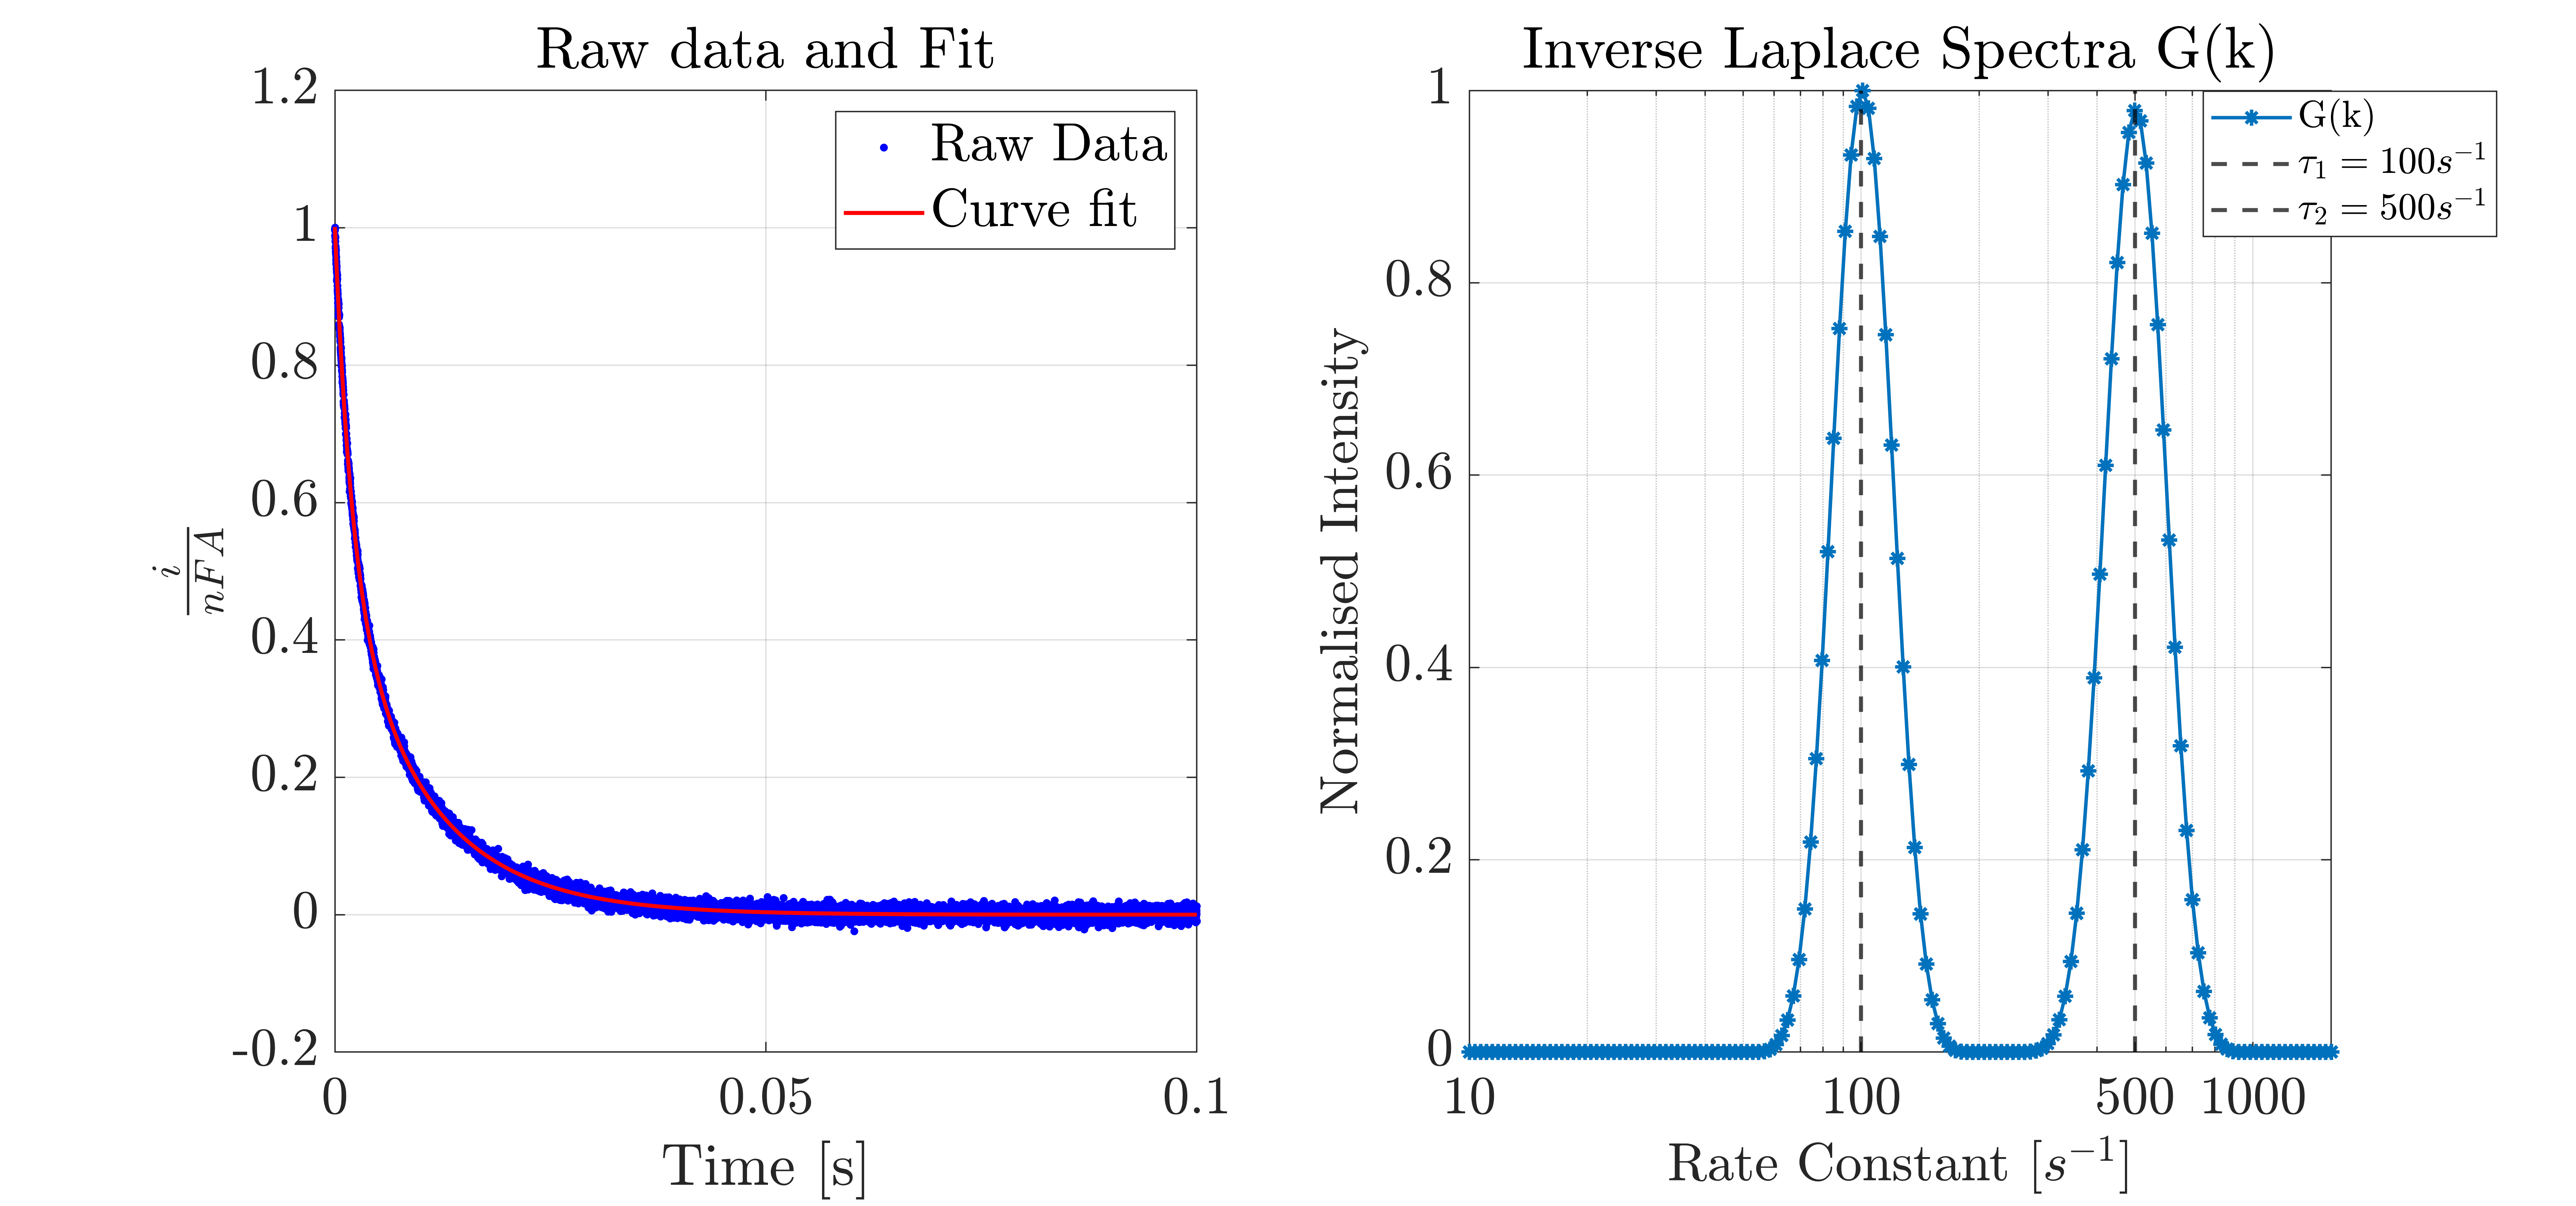
\includegraphics[width = 0.5\textwidth]{img/Inv_Laplace_results.png}
    \caption{Inverse Laplace Algorithm performance against simulated data with rate constants $k_{A} = 100s^{-1}$ and $k_{AT} = 500s^{-1}$}
    \label{multiexp}
\end{figure}
\begin{figure}[H]
    \centering
    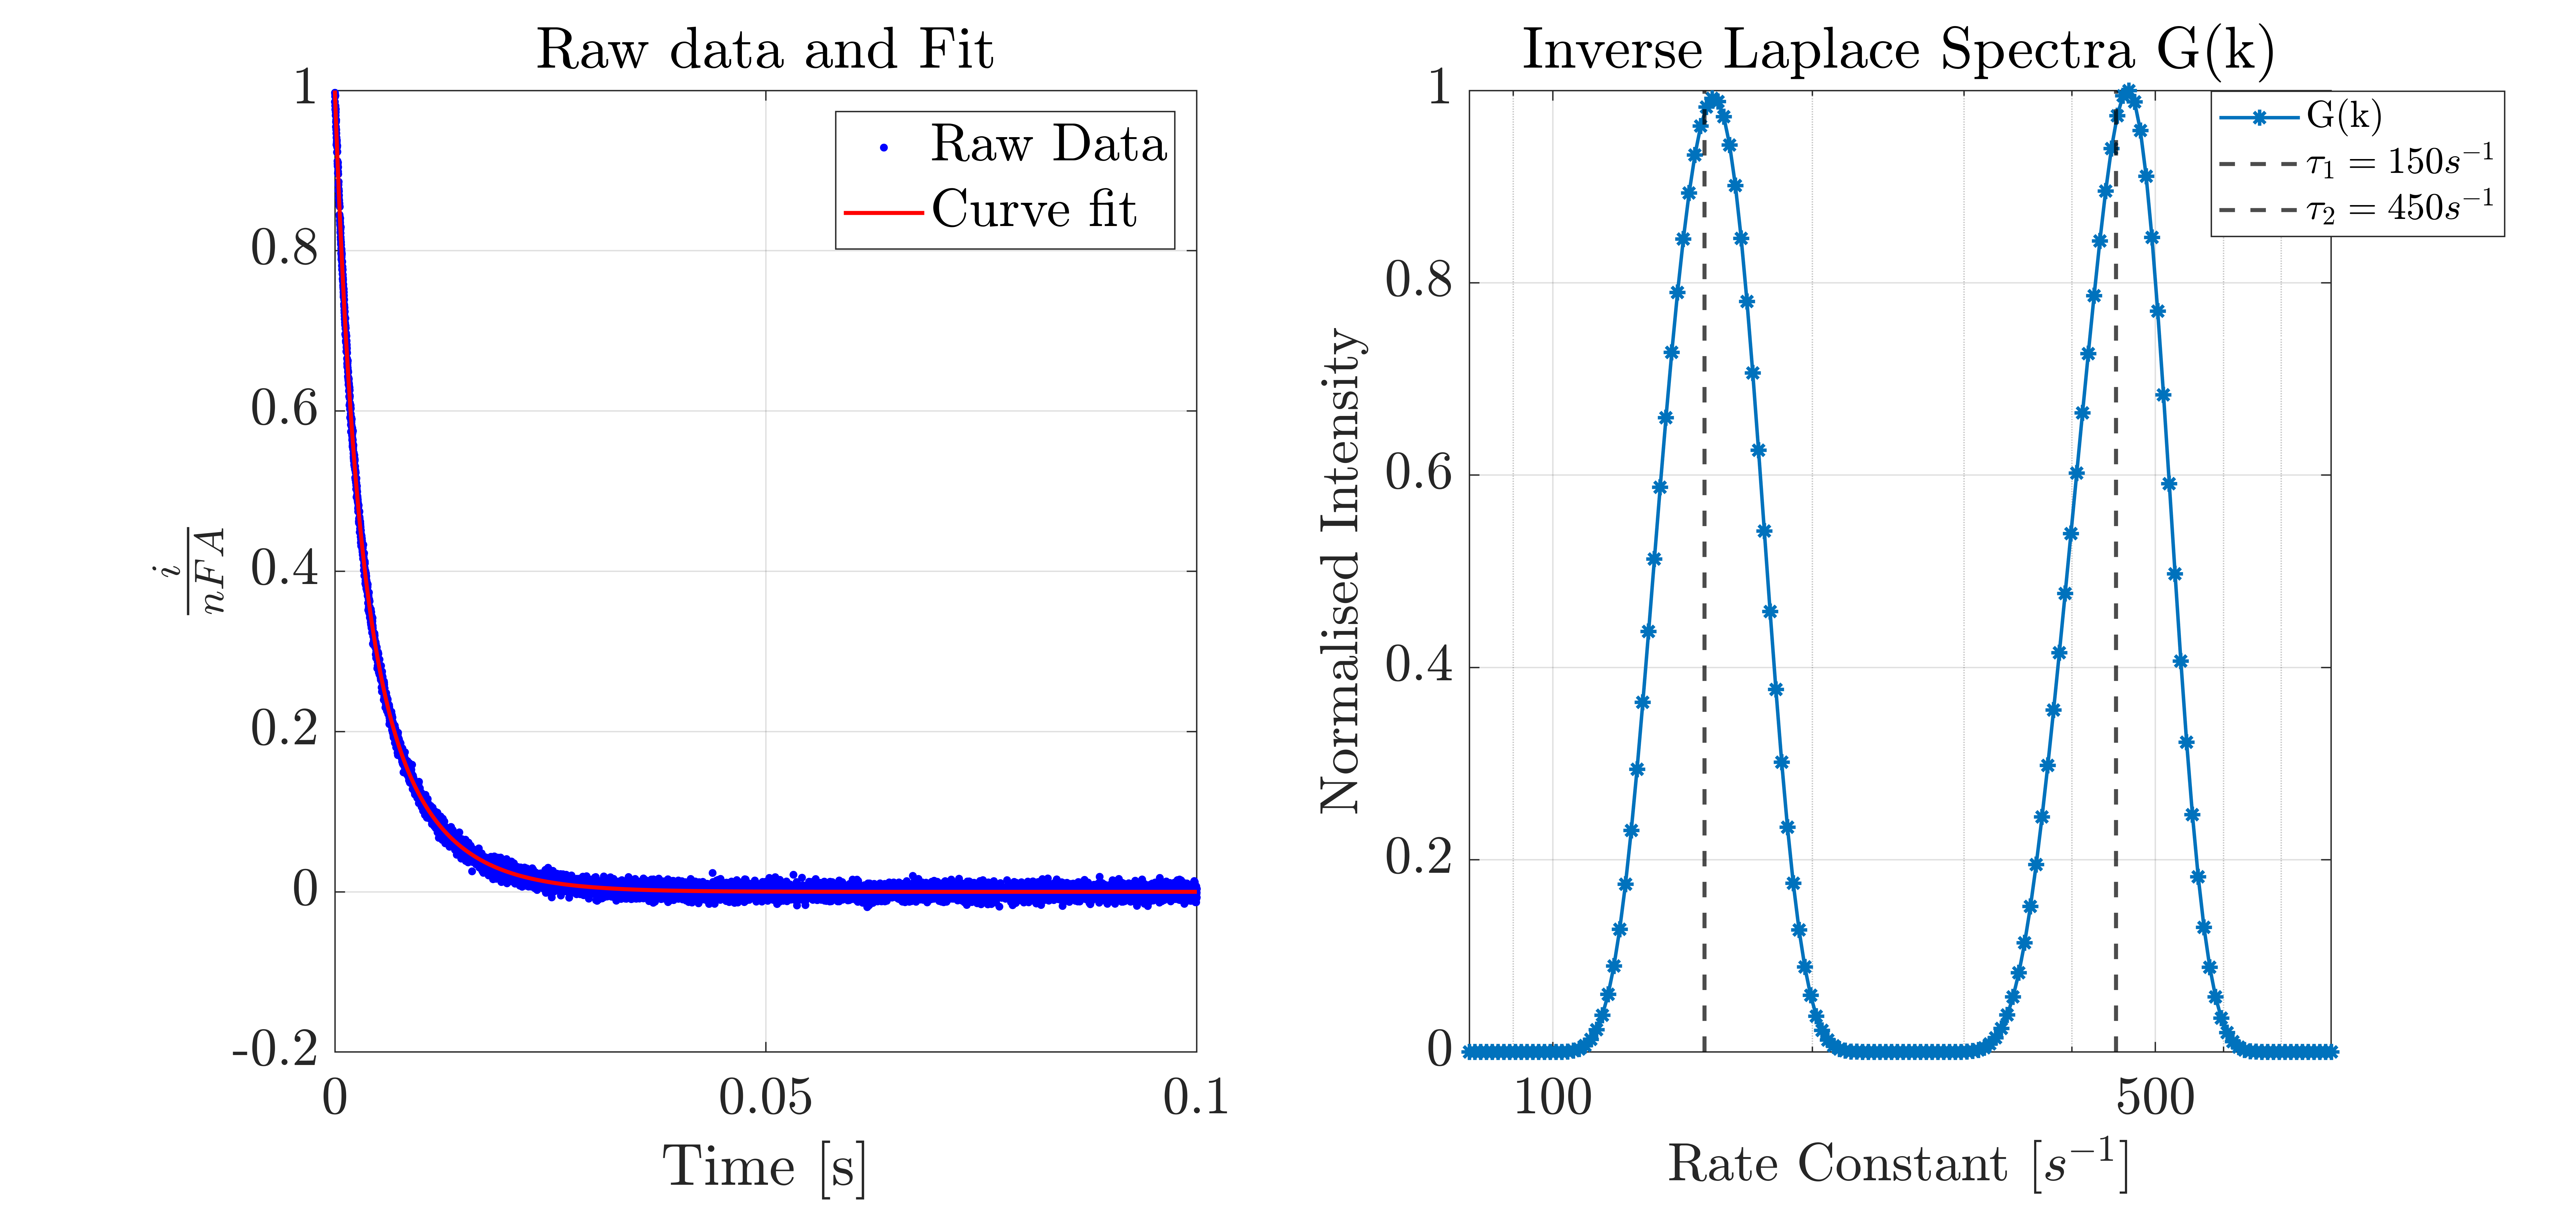
\includegraphics[width = 0.5\textwidth]{img/Inv_laplace_150_450.png}
    \caption{Inverse Laplace Algorithm performance against simulated data with rate constants $k_{A} = 150s^{-1}$ and $k_{AT} = 450s^{-1}$}
    \label{multiexp_2}
\end{figure}
\begin{figure}[H]
    \centering
    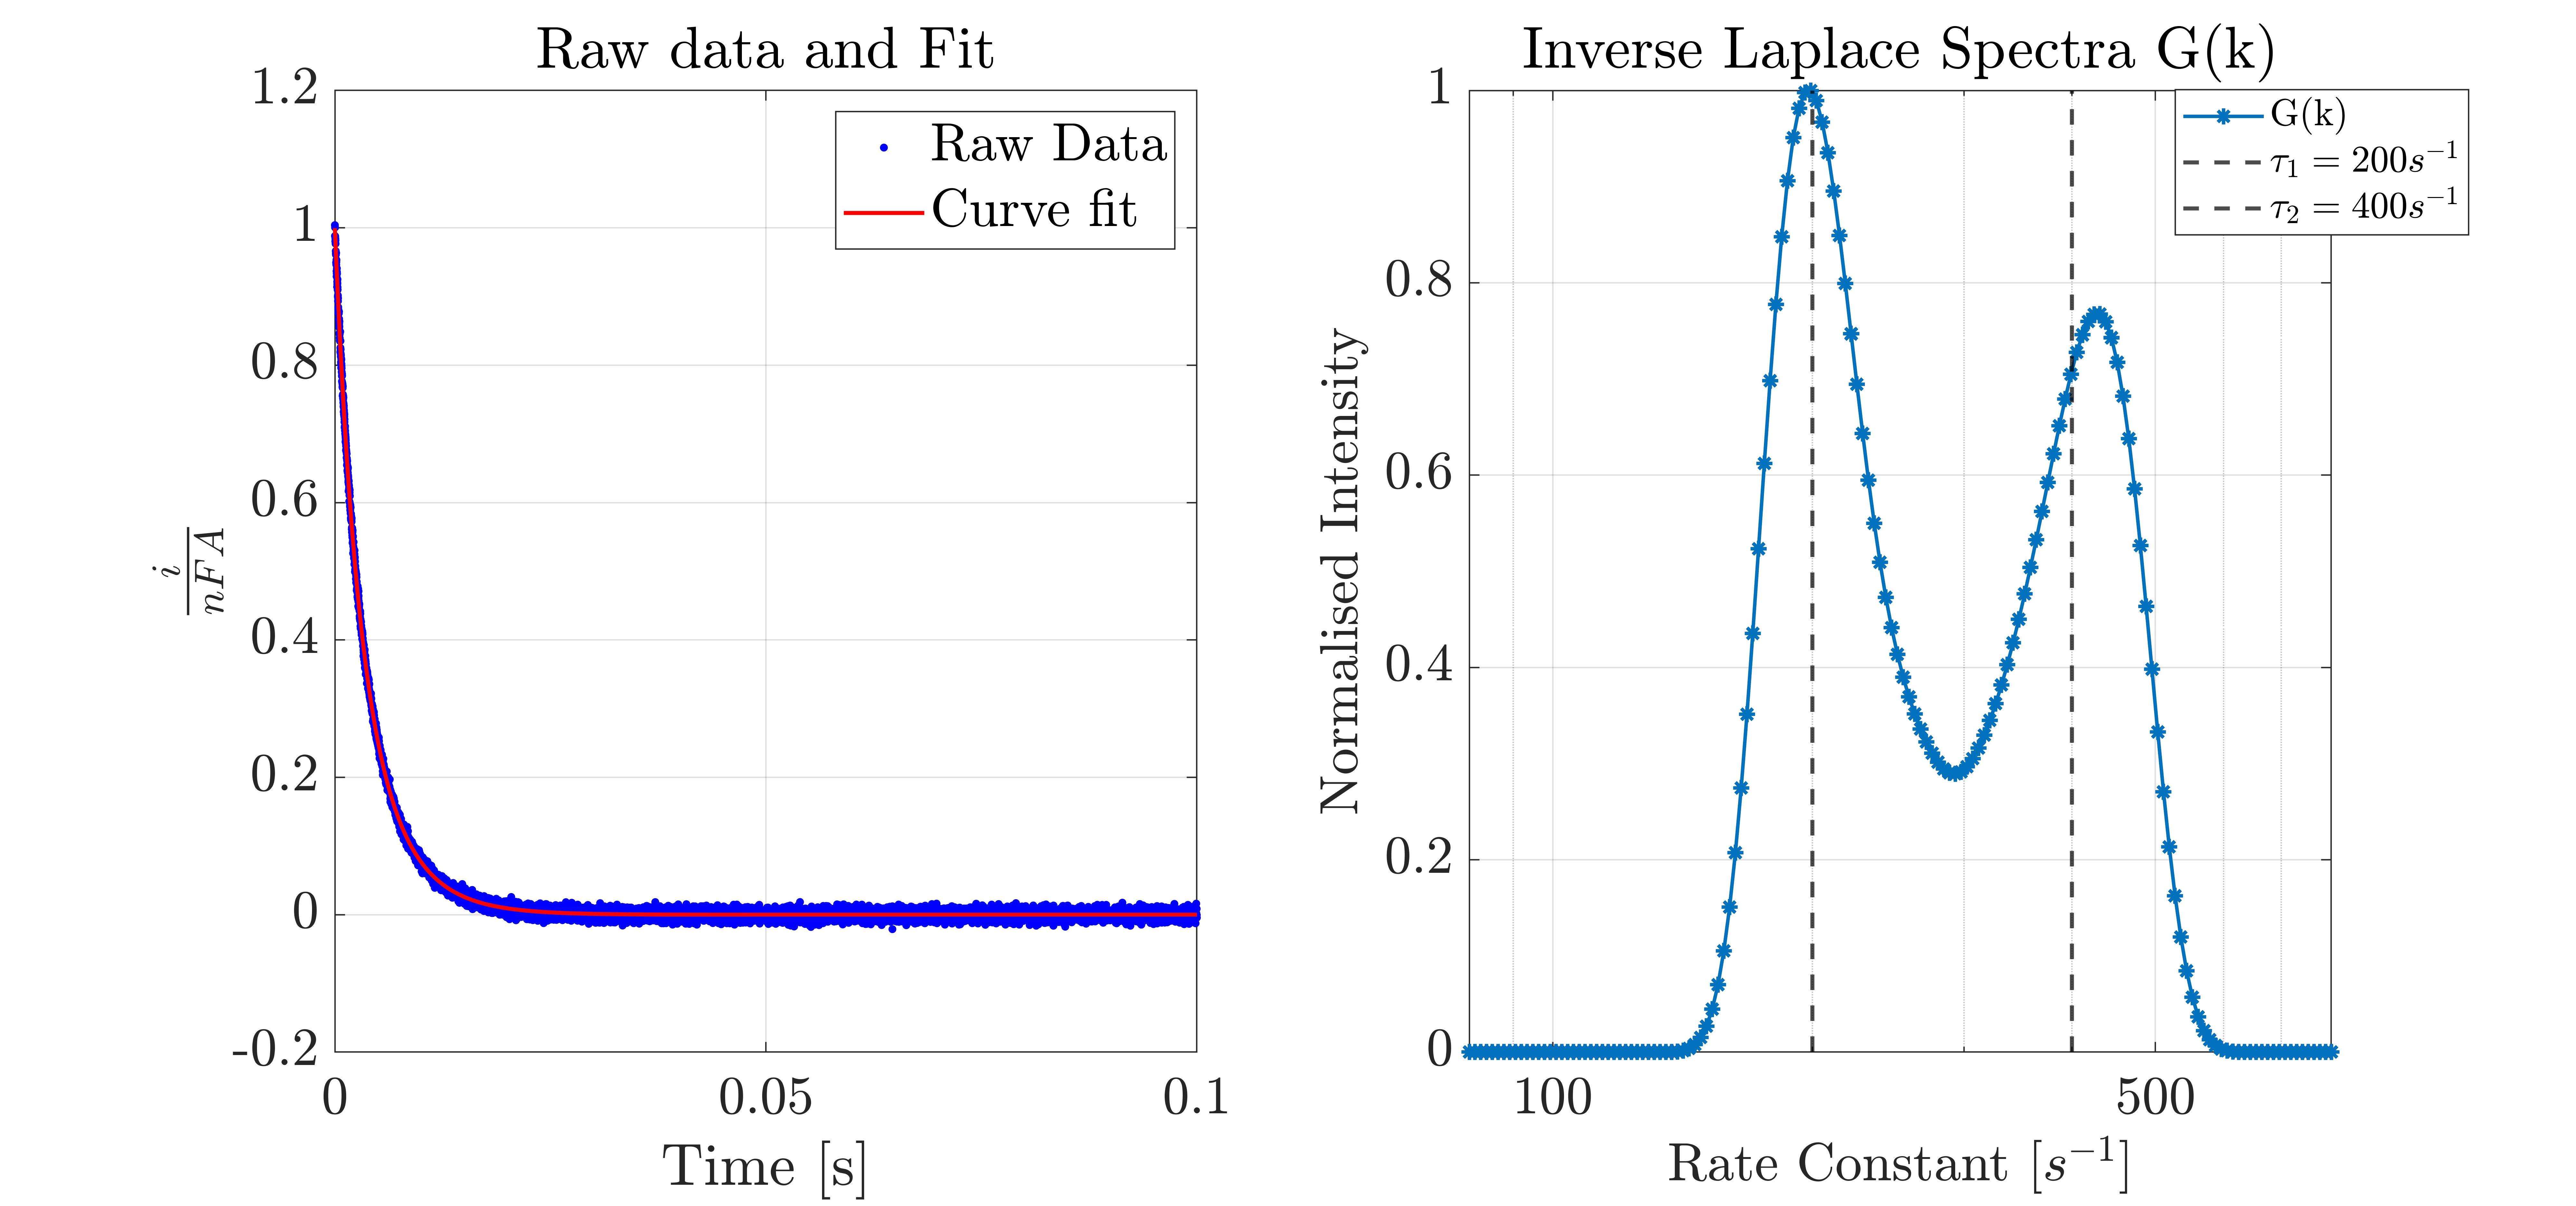
\includegraphics[width = 0.5\textwidth]{img/Inv_laplace_200_400.png}
    \caption{Inverse Laplace Algorithm performance against simulated data with rate constants $k_{A} = 200s^{-1}$ and $k_{AT} = 400s^{-1}$. Overlap in peaks, however can still distinguish the two peaks as distribution is bimodal.}
    \label{multiexp_3}
\end{figure}
\begin{figure}[H]
    \centering
    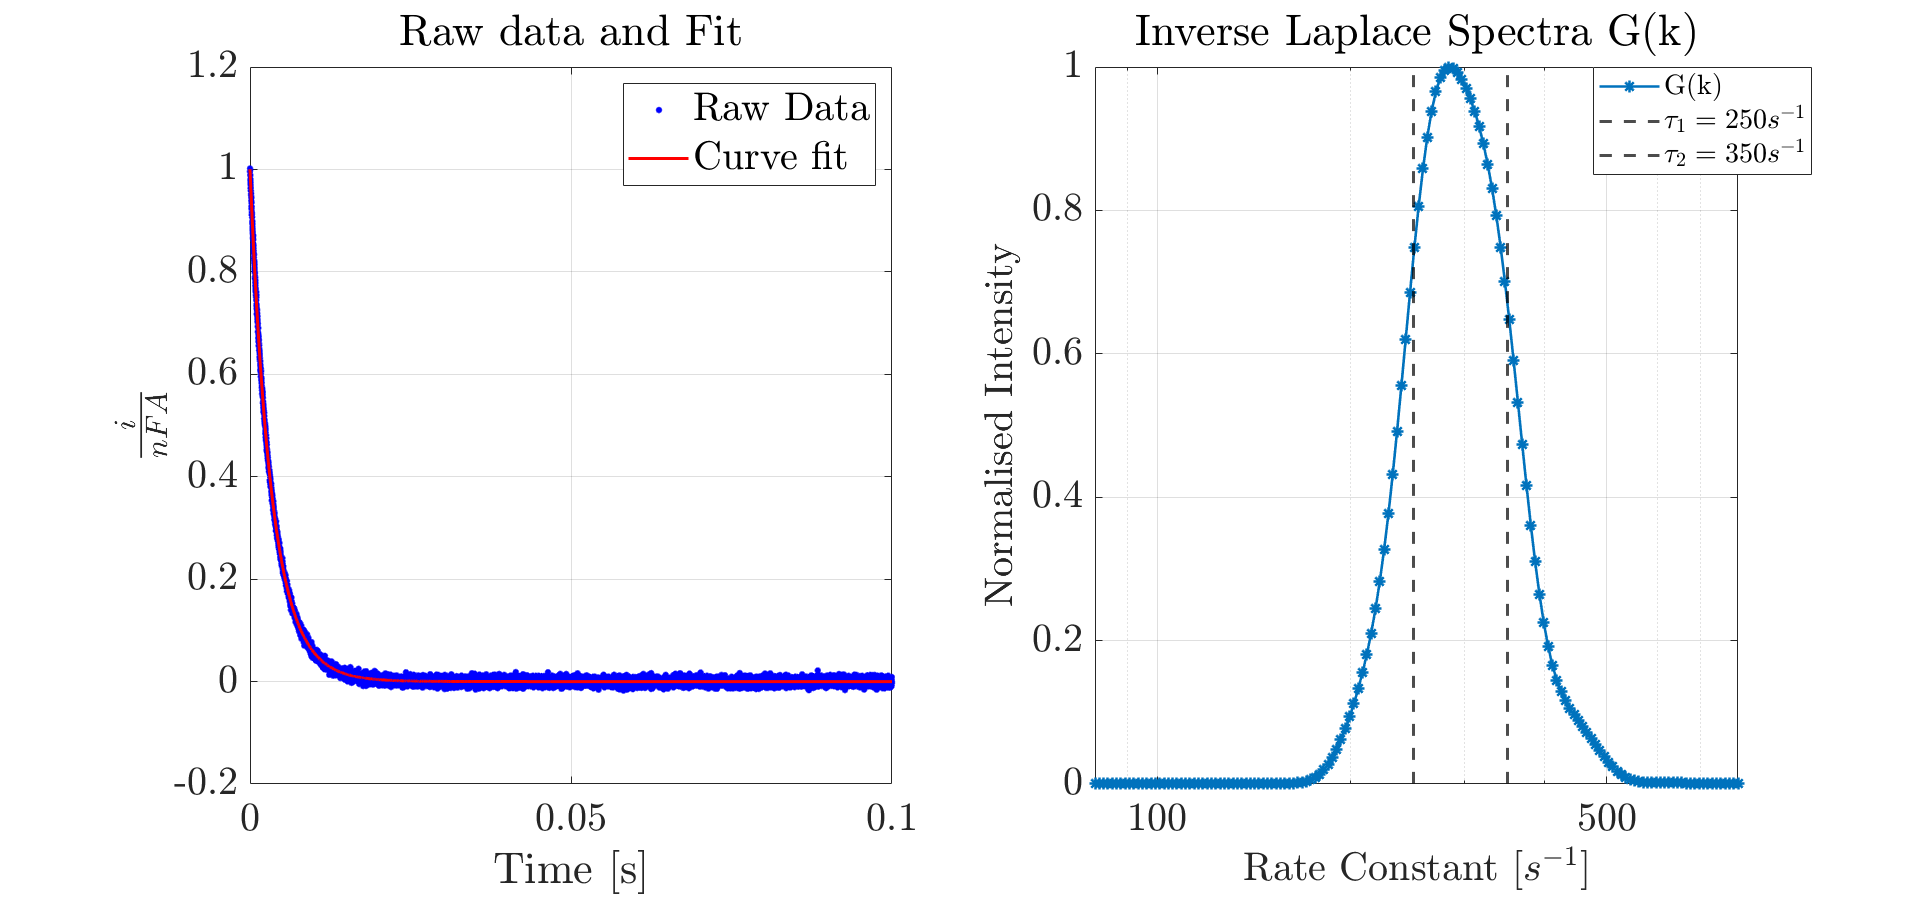
\includegraphics[width = 0.5\textwidth]{img/Inv_laplace_250_350.png}
    \caption{Inverse Laplace Algorithm performance against simulated data with rate constants $k_{A} = 250s^{-1}$ and $k_{AT} = 350s^{-1}$. The rate constants are close such that the two peaks have merged into one peak.}
    \label{multiexp_4}
\end{figure}
\subsection{Coarse-grained Aptamer Model Predictions}
Assuming electron transfer is effectively instantaneous at small distances in a Nernstian process through the SAM \cite{finklea1992electron,smalley1995kinetics}, we can use the collision model \cite{huang2013random} to estimate the probability for an electron transfer event from occurring for a given aptamer length. The length of a Methylene-Blue molecule is 14.47$\angstrom$ \cite{dotto2015adsorption}. This is equivalent to a distance of 1.45nm. Using this distance as the threshold value, we obtain the following probabilities that a collision occurs for the various aptamer lengths tested (\autoref{dep_plot_2}):
\begin{figure}[H]
    \centering
    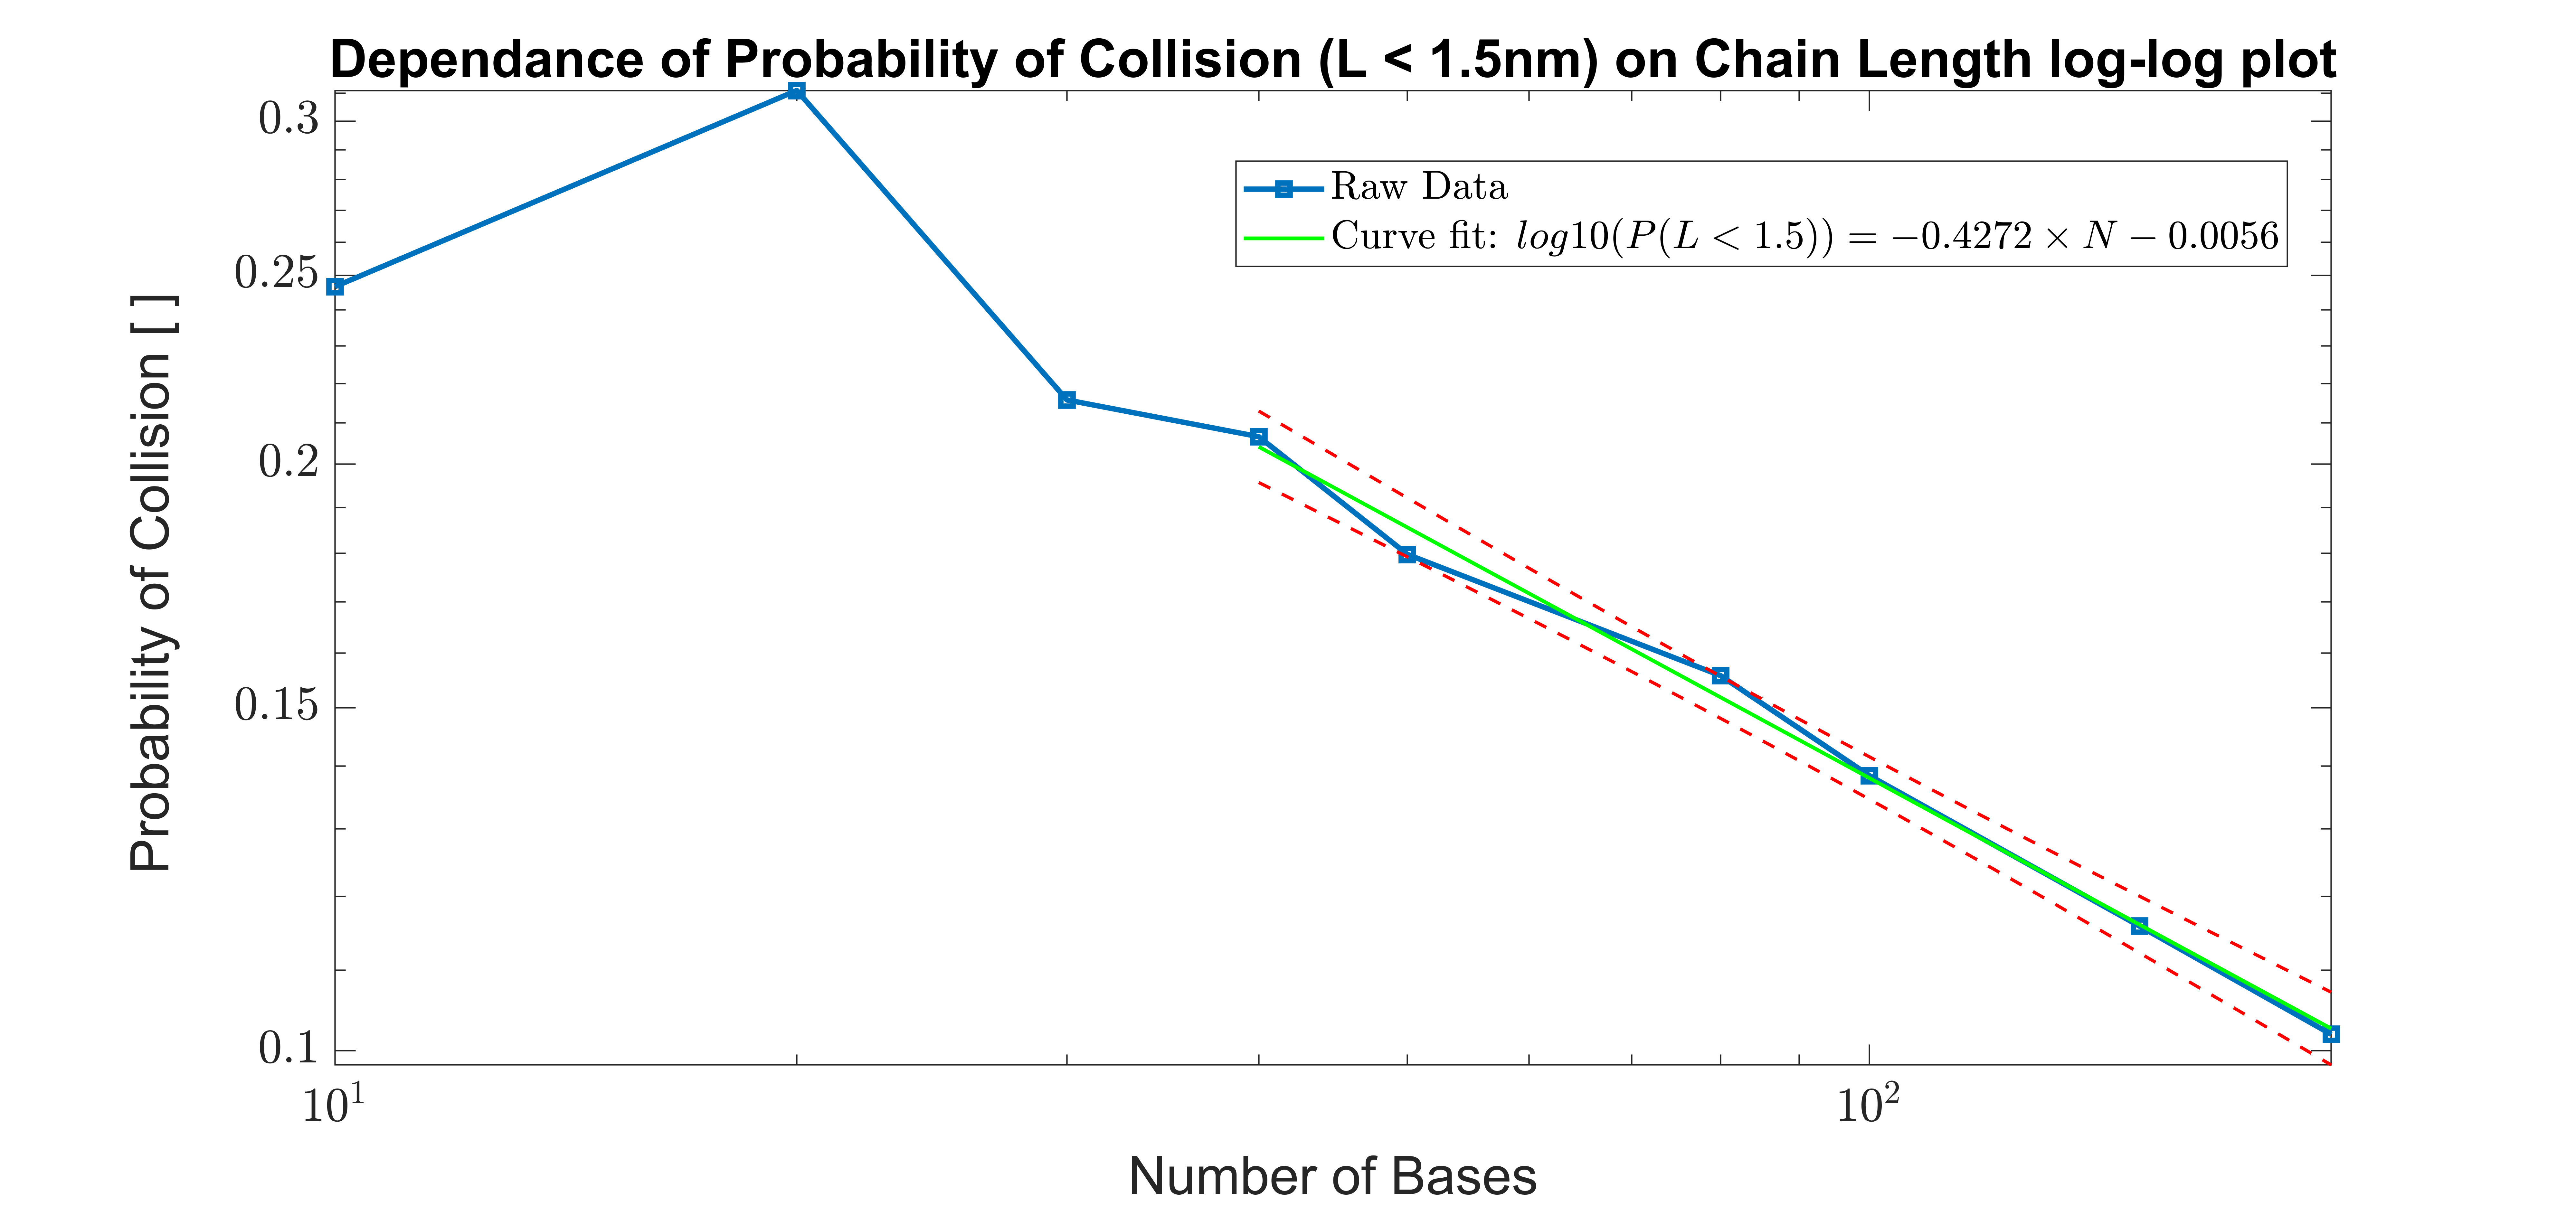
\includegraphics[width = 0.5\textwidth]{img/Length_dep_bases_log.png}
    \caption{Dependance of probability of collision (L $<$ 1.5nm) on the base length for the freely-jointed chain model of the aptamer. Log-log plot. Curve fit shows a -0.4272 dependence of log10(P$<$1.5nm) to log10(N) where N is the number of bases.}
    \label{dep_plot_2}
\end{figure}
\noindent{We can see that by plotting the length in a log scale, the collision probability has a linear dependence on the base length. These estimates are comparable to studies done by Plaxco et al. (\autoref{plaxco_plot} \cite{arroyo2018subsecond}) who found apparent electron transfer rate exhibits a power-law dependence on chain length, N (number of monomers)
with an exponent of 1.166 $\pm$ 0.09.}
\begin{figure}[H]
    \centering
    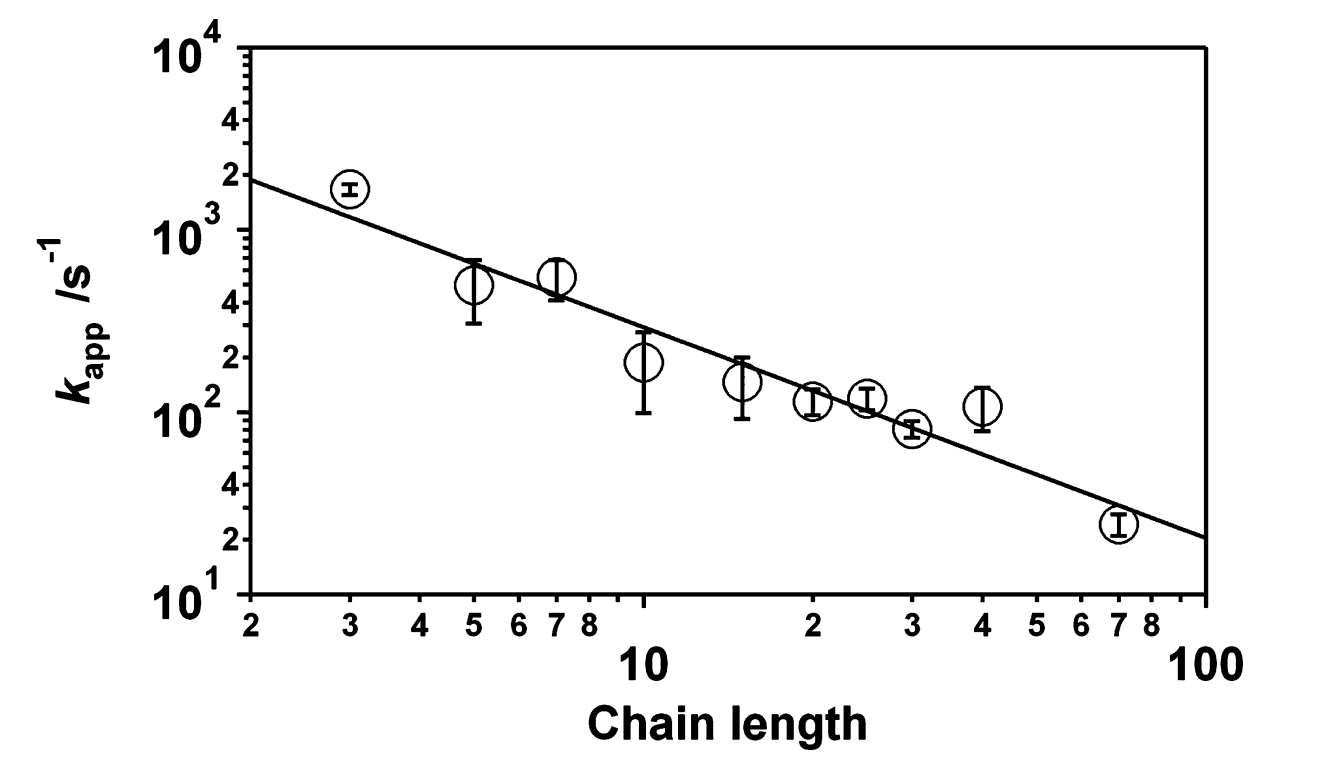
\includegraphics[width = 0.5\textwidth]{img/Plaxco_k_app_vs_length.png}
    \caption{Dependence of rate constant on the base length for the freely-jointed chain model of the aptamer. Log-log plot. The apparent electron transfer rate exhibits a power-law dependence on chain length, N (number of monomers) with an exponent of 1.166 $\pm$ 0.09. \cite{uzawa2010mechanistic}}
    \label{plaxco_plot}
\end{figure}
